% Version 1.2 of SN LaTeX, November 2022
%
% See section 11 of the User Manual for version history 
%
%%%%%%%%%%%%%%%%%%%%%%%%%%%%%%%%%%%%%%%%%%%%%%%%%%%%%%%%%%%%%%%%%%%%%%
%%                                                                 %%
%% Please do not use \input{...} to include other tex files.       %%
%% Submit your LaTeX manuscript as one .tex document.              %%
%%                                                                 %%
%% All additional figures and files should be attached             %%
%% separately and not embedded in the \TeX\ document itself.       %%
%%                                                                 %%
%%%%%%%%%%%%%%%%%%%%%%%%%%%%%%%%%%%%%%%%%%%%%%%%%%%%%%%%%%%%%%%%%%%%%

%%\documentclass[referee,sn-basic]{sn-jnl}% referee option is meant for double line spacing

%%=======================================================%%
%% to print line numbers in the margin use lineno option %%
%%=======================================================%%

%%\documentclass[lineno,sn-basic]{sn-jnl}% Basic Springer Nature Reference Style/Chemistry Reference Style

%%======================================================%%
%% to compile with pdflatex/xelatex use pdflatex option %%
%%======================================================%%

%%\documentclass[pdflatex,sn-basic]{sn-jnl}% Basic Springer Nature Reference Style/Chemistry Reference Style


%%Note: the following reference styles support Namedate and Numbered referencing. By default the style follows the most common style. To switch between the options you can add or remove “Numbered” in the optional parenthesis. 
%%The option is available for: sn-basic.bst, sn-vancouver.bst, sn-chicago.bst, sn-mathphys.bst. %  
 
%%\documentclass[sn-nature]{sn-jnl}% Style for submissions to Nature Portfolio journals
%%\documentclass[sn-basic]{sn-jnl}% Basic Springer Nature Reference Style/Chemistry Reference Style
\documentclass[sn-mathphys,Numbered]{sn-jnl}% Math and Physical Sciences Reference Style
%%\documentclass[sn-aps]{sn-jnl}% American Physical Society (APS) Reference Style
%%\documentclass[sn-vancouver,Numbered]{sn-jnl}% Vancouver Reference Style
%%\documentclass[sn-apa]{sn-jnl}% APA Reference Style 
%%\documentclass[sn-chicago]{sn-jnl}% Chicago-based Humanities Reference Style
%%\documentclass[default]{sn-jnl}% Default
%%\documentclass[default,iicol]{sn-jnl}% Default with double column layout

%%%% Standard Packages
%%<additional latex packages if required can be included here>

\usepackage{graphicx}%
\usepackage{multirow}%
\usepackage{amsmath,amssymb,amsfonts}%
\usepackage{amsthm}%
\usepackage{mathrsfs}%
\usepackage[title]{appendix}%
\usepackage{xcolor}%
\usepackage{textcomp}%
\usepackage{manyfoot}%
\usepackage{booktabs}%
\usepackage{algorithm}%
\usepackage{algorithmicx}%
\usepackage{algpseudocode}%
\usepackage{listings}%
\usepackage{xcolor}
%%%%
%\usepackage{caption}
%\linespread{2.5} % Adds line spacing across the overleaf document

%%%%%=============================================================================%%%%
%%%%  Remarks: This template is provided to aid authors with the preparation
%%%%  of original research articles intended for submission to journals published 
%%%%  by Springer Nature. The guidance has been prepared in partnership with 
%%%%  production teams to conform to Springer Nature technical requirements. 
%%%%  Editorial and presentation requirements differ among journal portfolios and 
%%%%  research disciplines. You may find sections in this template are irrelevant 
%%%%  to your work and are empowered to omit any such section if allowed by the 
%%%%  journal you intend to submit to. The submission guidelines and policies 
%%%%  of the journal take precedence. A detailed User Manual is available in the 
%%%%  template package for technical guidance.
%%%%%=============================================================================%%%%

%\jyear{2021}%

%% as per the requirement new theorem styles can be included as shown below
\theoremstyle{thmstyleone}%
\newtheorem{theorem}{Theorem}%  meant for continuous numbers
%%\newtheorem{theorem}{Theorem}[section]% meant for sectionwise numbers
%% optional argument [theorem] produces theorem numbering sequence instead of independent numbers for Proposition
\newtheorem{proposition}[theorem]{Proposition}% 
%%\newtheorem{proposition}{Proposition}% to get separate numbers for theorem and proposition etc.

\theoremstyle{thmstyletwo}%
\newtheorem{example}{Example}%
\newtheorem{remark}{Remark}%

\theoremstyle{thmstylethree}%
\newtheorem{definition}{Definition}%

\raggedbottom
%%\unnumbered% uncomment this for unnumbered level heads

\begin{document}

%\title[Article Title]{Developing Comprehensive Annotation Guidelines and a Corpus of Risk of Bias Assessment for Rehabilitation: A Methodological Approach}
\title[Article Title]{RoBuster: A Corpus Annotated with Risk of Bias Text Spans in Randomized Controlled Trials}

%%=============================================================%%
%% Prefix	-> \pfx{Dr}
%% GivenName	-> \fnm{Joergen W.}
%% Particle	-> \spfx{van der} -> surname prefix
%% FamilyName	-> \sur{Ploeg}
%% Suffix	-> \sfx{IV}
%% NatureName	-> \tanm{Poet Laureate} -> Title after name
%% Degrees	-> \dgr{MSc, PhD}
%% \author*[1,2]{\pfx{Dr} \fnm{Joergen W.} \spfx{van der} \sur{Ploeg} \sfx{IV} \tanm{Poet Laureate} 
%%                 \dgr{MSc, PhD}}\email{iauthor@gmail.com}
%%=============================================================%%

\author*[1,2]{\fnm{Anjani} \sur{Dhrangadhariya}}\email{anjani.dhrangadhariya@hevs.ch}

\author[3]{\fnm{Roger} \sur{Hilfiker}}\email{roger.hilfiker@proton.me}

\author[4]{\fnm{Martin} \sur{Sattelmayer}}\email{martin.sattelmayer@hevs.ch}

\author[5,6]{\fnm{Nona} \sur{Naderi}}\email{nona.naderi@hesge.ch}

\author[4]{\fnm{Katia} \sur{Giacomino}}\email{katia.giacomino@hevs.ch}
\equalcont{These authors contributed equally to this work.}

\author[4]{\fnm{Rahel} \sur{Caliesch}}\email{rahel.caliesch@hevs.ch}
\equalcont{These authors contributed equally to this work.}

\author[1]{\fnm{Stéphane} \sur{Marchand-Maillet}}\email{stephane.marchand-maillet@unige.ch}

\author[1,2]{\fnm{Henning} \sur{Müller}}\email{henning.mueller@hevs.ch}


\affil*[1]{\orgdiv{Department of Computer Science}, \orgname{University of Geneva}, \orgaddress{\city{Geneva}, \country{Switzerland}}}

\affil[2]{\orgdiv{Informatics Institute}, \orgname{HES-SO Valais-Wallis}, \orgaddress{\city{Sierre}, \country{Switzerland}}}

\affil[3]{\orgdiv{IUFRS}, \orgname{University of Lausanne}, \orgaddress{\city{Lausanne}, \country{Switzerland}}}

\affil[4]{\orgdiv{School of Health Sciences}, \orgname{HES-SO Valais-Wallis}, \orgaddress{\city{Leukerbad}, \country{Switzerland}}}

\affil[5]{\orgdiv{Geneva School of Business Administration}, \orgname{HES-SO Geneva}, \orgaddress{\city{Geneva}, \country{Switzerland}}}

\affil[6]{\orgname{Swiss Institute of Bioinformatics (SIB)}, \orgaddress{\city{Geneva}, \country{Switzerland}}}

%%==================================%%
%% sample for unstructured abstract %%
%%==================================%%
% Do not go beyond 200 words for the abstract.
%\abstract{The abstract serves both as a general introduction to the topic and as a brief, non-technical summary of the main results and their implications. Authors are advised to check the author instructions for the journal they are submitting to for word limits and if structural elements like subheadings, citations, or equations are permitted.}

%%================================%%
%% Sample for structured abstract %%
%%================================%%

\abstract{\textbf{Purpose:} Risk of bias (RoB) assessment of randomized clinical trials (RCTs) is vital to accurately answer a systematic review question.
Manual RoB assessment for hundreds of clinical trials is a cognitively demanding and lengthy process.
Automation has the potential to assist reviewers in rapidly identifying text descriptions in RCTs that indicate potential bias.
However, there is no annotated corpus for RoB to fine-tune large language models (LLMs) and no established guidelines for annotating the risk of bias in RCTs.
% 
\textbf{Methods:} We utilized the revised Cochrane Risk of Bias Assessment 2 guidelines for RCTs to create visual instructional placards serving as text annotation guidelines for RoB spans and risk judgments.
Expert annotators employed these visual guidelines to annotate a corpus of 41 full-text RCTs from physiotherapy and rehabilitation.
We report inter-annotator agreements (IAA) at two levels: agreement on text spans and risk judgments between two expert annotators when applying the guidelines to a subset (9 out of 41) of the annotated corpus.
Additionally, a portion of the corpus (10 out of 40) was employed to evaluate an LLM using a straightforward evaluation framework.
% 
\textbf{Results:} We present a corpus of 41 RCTs with fine-grained text span annotations comprising more than 28,427 tokens belonging to 22 RoB classes.
The IAA at the text span level varies from $0\%$ to $90\%$, while the IAA for risk judgments ranges between $-0.235$ and $1.0$.
LLMs show promising but variable observed agreements with the expert annotation across the different bias questions.
% 
\textbf{Conclusion:} 
Despite having comprehensive bias assessment guidelines and visual instructional placards, RoB annotation remains a complex task.
Utilizing visual placards for bias assessment and annotation enhances IAA compared to cases where visual placards are absent.
However, text annotation remains challenging for the subjective, low information availability questions.
While LLMs demonstrate efficacy, their accuracy diminishes with more subjective RoB questions and instances where RCT data is unavailable.}

\keywords{risk of bias, dataset, natural language processing, large language models}

%%\pacs[JEL Classification]{D8, H51}

%%\pacs[MSC Classification]{35A01, 65L10, 65L12, 65L20, 65L70}

\maketitle


%%%%%%%%%%%%%%%%
%% Background %%
\section{Background and Significance}
\label{sec:background}
%
Systematic reviews (SRs) synthesized using randomized controlled trials (RCTs) are the highest quality of evidence in the evidence pyramid.
SRs aid medical professionals make educated decisions about an individual's health and help governments enact informed health policies~\cite{mogo2022systematic,mctigue2006obesity}.
An RCT is a scientific experiment aiming to evaluate the efficacy of an intervention on particular patient outcomes.
In these trials, patients are randomly divided and allocated to either an active intervention group or a comparator group, and the impact of intervention compared to the comparator is measured in a controlled setting~\cite{sibbald1998understanding}.
Theoretically, RCTs are low on biases given the randomized study design but are still prone to unavoidable biases creeping into the trial's design, execution, or reporting.
Biased clinical trials make medical practitioners systematically overestimate or underestimate the intervention effect on patient outcomes, leading to harmful health practices and policies~\cite{kjaergard1999randomized,naci2019design}.
Thus, reviewers conducting SRs must thoroughly screen RCTs for biases before inclusion in writing SRs.


The biases in RCTs cannot be quantified, but an RCT can be assessed for biases to minimize the overall risk and judge its quality.
In this study, we refer to bias assessment as risk-of-bias (RoB) assessment.
There are several tools to assess RoB, including the Cochrane Collaborations RoB Tool, Physiotherapy Evidence Database (PEDro) RoB scale, revised Cochrane RoB 2 tool (RoB 2), AMSTAR/AMSTAR 2, EPOC RoB Tool and several other independent checklists~\cite{higgins2019,higgins2011cochrane,elkins2013growth,sterne2019rob,shea2017amstar,farrah2019risk}.
These tools are structured as a series of questions aiming to elicit factual information from the RCTs, which could then be used for RoB assessment.
%These tools are a series of questions aiming to elicit factual information from the RCTs, which can then be used to assess their quality.
Manual quality assessment requires the reviewers to go through full-text RCTs and manually inspect every question from the chosen bias assessment tool.
The process takes about 3-10 months per person per SR and requires a high degree of methodological expertise on the reviewer's part.
Moreover, RoB assessment is a part of writing systematic reviews, which is highly resource-heavy, taking about six months to several years to complete the review~\cite{tsertsvadze2015conduct,khangura2012evidence,higgins2019cochrane}.
The pace at which RCTs are published makes RoB assessment a lengthy process and underscores the need for automation.



Machine learning (ML) can help accelerate the assessment process by directly pointing the reviewers to the parts of the RCT text relevant to identifying bias, leading to quickly judging the trial quality.
Marshall \textit{et al.}~\cite{marshall2015automating} attempted automation of RoB assessment using distant supervision approach supported by proprietary data from the Cochrane Database of Systematic Reviews (CDSR). 
They formulated the trial quality assessment as binary classification into \textit{low-risk} and \textit{unclear-risk/high-risk} quality attributes for each risk domain.
The study was supported by the manually-entered data from CDSR, which is behind a paywall and automates based on Cochrane's RoB 1.0 guidelines and not the latest RoB 2~\cite{higgins2011cochrane}.
Even though Cochrane's RoB tool (version 1) is the most frequently used to assess RCT quality, a recently revised Cochrane RoB 2 offers significant differences in comparison~\cite{ma2020methodological}.
Compared to the original RoB version released in 2008, the RoB 2 version provides a more reliable and concrete structure to the RoB evaluation by developing comprehensive guidelines that enforce consistency~\cite{higgins2011cochrane,sterne2019rob}.
A study analyzing Cochrane systematic reviews and protocols found that the use of RoB 2 increased from 0\% in 2019 to 24.1\% in 2022~\cite{martimbianco2023most}.
This indicates the importance of using an updated and standardized tool to assess bias in RCTs.

Millard \textit{et al.} attempted automating RoB assessment using supervised machine learning trained on proprietary data as well~\cite{millard2016machine}.
In fact, the research utilising this pay-walled data was used to develop RobotReviewer that has been evaluated by several studies for its human-competent performance~\cite{marshall2016robotreviewer,soboczenski2019machine,vinkers2021methodological,jardim2022automating,hirt2021agreement}.
The question, however, remains of the unavailability of a publicly-available RoB annotated corpus that hinders community efforts for automation. 
Wang \textit{et al.} recently released three RoB annotated datasets, but for preclinical animal studies with RoB assessments pertaining to animals~\cite{wang2022risk}.
A manually annotated corpus of RoB spans for human clinical trials is still necessary.
Manual RoB assessment is a complex, expert-led task laden with subjective judgements.
Systematically translating this manual process for developing an RoB annotated corpus requires a carefully designed annotation scheme and detailed annotation guidelines.
Recently Dhrangadhariya \textit{et al.} worked on a pilot study to test whether RoB 2 guidelines could be effectively utilized as guidelines to manually annotate a corpus of RCTs with RoB using a multi-level annotation scheme adapted from the same guidelines.
They conclude that the assesment guidelines cannot be used as text annotation guidelines, but neither provide any annotation guidelines from their end.
Additionally, the dataset they provide is comparatively small with 10 annotated RCTs~\cite{dhrangadhariya2023first}.
Our objective is to develop clear cut annotation guidelines to annotate RCTs with RoB spans corresponding to RoB 2 tool for randomized controlled trials~\cite{sterne2019rob}.



Recently, large language models (LLMs) have demonstrated exceptional performance on unseen tasks when only the task instructions are provided~\cite{chang2023survey}.
However, till date, no one has evaluated their performance on the cognitively complex task of identifying RoB text descriptions from RCTs and providing their RCT quality judgments based on text.
Our contributions with this paper are five-fold. 
1) We develop comprehensive annotation guidelines for annotating RCTs with risk of bias description.
2) We model these annotation guidelines in form of visual placards for ease of annotation and understanding. These placards could be used as visual RoB assessment guidelines by the trainee RoB assessors.
3) We annotate a corpus of 41 full-text RCTs with 22 risk of bias span types which could be used to fine-tune machine learning models or LLMs and could also be used as a validation benchmark.
4) We evaluate the performance of LLMs to automatically identify the answers to these signalling questions (SQs) using prompt generation.
5) We make the visual annotation guidelines, the dataset and LLM prompts openly-available for the scientific community.
%
%
%
\section{Methodology}
\label{sec:methods}
%
This section describes the annotation scheme, annotation softwares and visual placard development.
Since there are no text annotation guidelines available for RoB span annotation task, we take pleasure in formulating them from scratch using the revised Cochrane RoB 2 tool.
We first developed a draft version of our visual annotation guidelines, doubly annotated a fraction of documents using it and used the conflicts identified during this exercise to refine the guidelines.
%
%
%
\subsection{Annotation scheme}
\label{met:annot_scheme}
%

%
%
%
\begin{figure}
    \centering
    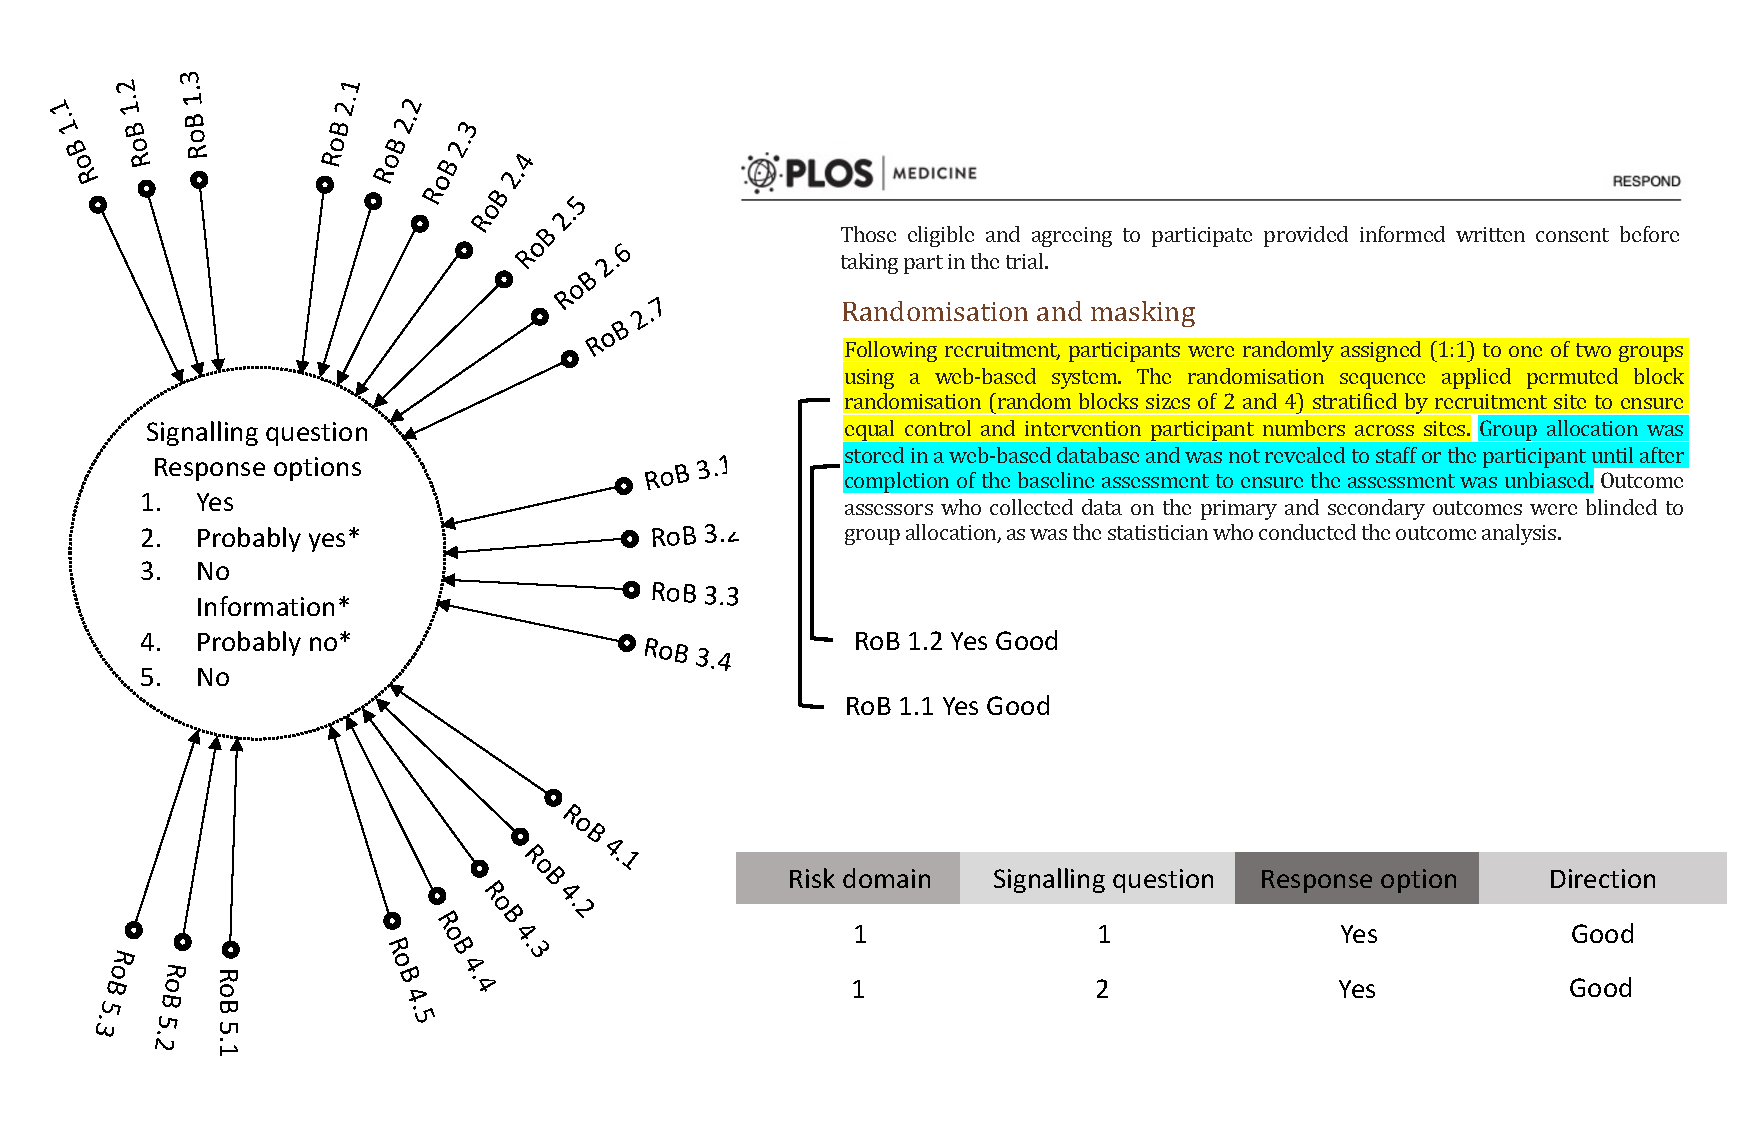
\includegraphics[width=0.99\columnwidth]{figures/annotation_schema.pdf}
    \caption{Our annotation scheme}
    \label{fig:annotationscheme}
\end{figure}
%
%
%



Creating a new annotated corpus involves defining an annotation scheme or adopting an existing one.
To our knowledge the only available annotation scheme for RoB span annotation was presented by~\cite{dhrangadhariya2023first}.
We adapt and enhance their approach by learning from its drawbacks rather than developing a new scheme.
Their annotation scheme was directly adapted from the RoB 2 assessment procedure and hence it is imperative to understand the RoB 2 organization to understand the annotation scheme.
RoB 2 divides biases into five risk domains, each loosely corresponding to different parts of the clinical trial design.
Each risk domain decomposes into several SQs, each aiming to prompt the assessor to look for relevant RCT text evidence and elicit a relevant response for bias risk judgment for that SQ (refer to Table~\ref{tab:robdomains}).


%
%
%
\begin{table*}
 \centering
 %\captionsetup{justification=justified}
   \caption{The table lists down the bias domains as structured in the revised Cochrane RoB assessment tool (RoB 2) and the number of signalling questions (SQs) in each domain.}\label{tab:robdomains}
    \begin{tabular}{llr}
    \toprule[1.0pt]
     Class & Domain & SQ\\
    \midrule[1.0pt]
    RoB 1 & biases arising from the \textbf{randomization process} &  3\\
    RoB 2 & biases due to \textbf{deviations from intended interventions} & 7\\
    RoB 3 & bias due to \textbf{missing outcome data} & 4\\
    RoB 4 & bias in the \textbf{measurement of the outcome} & 5\\
    RoB 5 & bias in the \textbf{selection of the reported result} & 3\\
    \bottomrule[1.0pt]
    \end{tabular}
\end{table*}
%
%
%


The response options for bias risk (or simply risk) judgment are restricted to ``Yes'', ``Probably yes'', ``No'', ``Probably no'', or ``No information''~\cite{sterne2019rob}.
Reviewers assess these SQs by examining the factual evidence in the RCT.
For instance, to answer the SQ ``Was the allocation sequence random?'', the reviewer reads through the RCT to identify how participants were randomized into intervention groups.
If a well-executed method of randomization is identified, the reviewer answers with ``yes'' (the allocation sequence is random) judging the risk of bias for this signaling question as low risk.
Conversely, if a poorly executed method of randomization is found, the risk of bias is deemed  high risk with response option ``no''.
%Similarly, each SQ prompts the reviewer to look for a piece(s) of factual evidence in the clinical study to respond with one of the five response options.



In RoB span annotation, we mimic this assessment process by considering evidence text spans in the RCT as the main units of annotation.
Each span corresponds to answering a SQ and is annotated with the most informative label. 
In our adopted annotation scheme, the label incorporates information about the SQ number and the domain it assesses (for the above example, ``1.1'' for the first domain and first SQ of the domain)
Additionally, the response option or risk judgement is incorporated in the label, such as ``1.1 Yes Good'' for a well-executed randomization procedure and ``1.1 No Bad'' otherwise (see Figure~\ref{fig:annotationscheme}).
Dhrangadhariya \textit{et al.} suggests collapsing the response options ``Yes'' and ``Probably Yes'' into a single ``Yes'', and ``No'' and ``Probably No'' together into a single ``No'' to increase the inter-annotator agreement (IAA) without altering the final risk domain judgment~\cite{dhrangadhariya2023first}.
As shown in Figure~\ref{fig:flowchart} responding to any SQ for the risk domain 2 as either ``Probably Yes'' or ``Yes'' does not alter the final risk judgment for this domain (low, high, or some concerns).
Therefore, except for some special case SQs, we too collapse these response option as suggested.
%In summary, the reviewer needs to label the identified text span with the RoB entity along with one of the response options.
In this regard, we have a hierarchical span annotation scheme comprising 22 entities corresponding to the 22 SQs, each with typically two response options (``Yes'' or ``No'') and two directions (``good'' and ``bad'').
We also remove the ``No Information'' response option because this was meant for the situations where actually no text evidence is found in the RCT to answer and label for a SQ.
However, for selected SQs, ``Probably Yes'', ``Probably No'' and ``No Information'' may still be acceptable.
For instance, consider that an RCT uses ``...random number generator and sealed envelopes for patient randomization...'', but the trial provided no information on whether the envelop was ``opaque'' or not.
%In such situations, ``No Information'' judgment is acceptable.
%Additionally, it is based on this span, the response judgment option is decided, and therefore even the response judgement information is incorporated in the label.
%Consider the following span is found to answer the above-mentioned SQ, ``randomized participants using random number generation...'', which is a good randomization procedure and therefore the reviewer responds with ``yes''.
%The label extends the example label to ``1.1 Yes''.
%In addition, a direction is also added to the label, for example, whether it is ``good'' or ``bad.
%In this example, a good randomization ensure low risk for this SQ and vice versa.
%Adding direction extends the example label to ``1.1 Yes Good''.


%
%
%
\begin{figure}
    \centering
    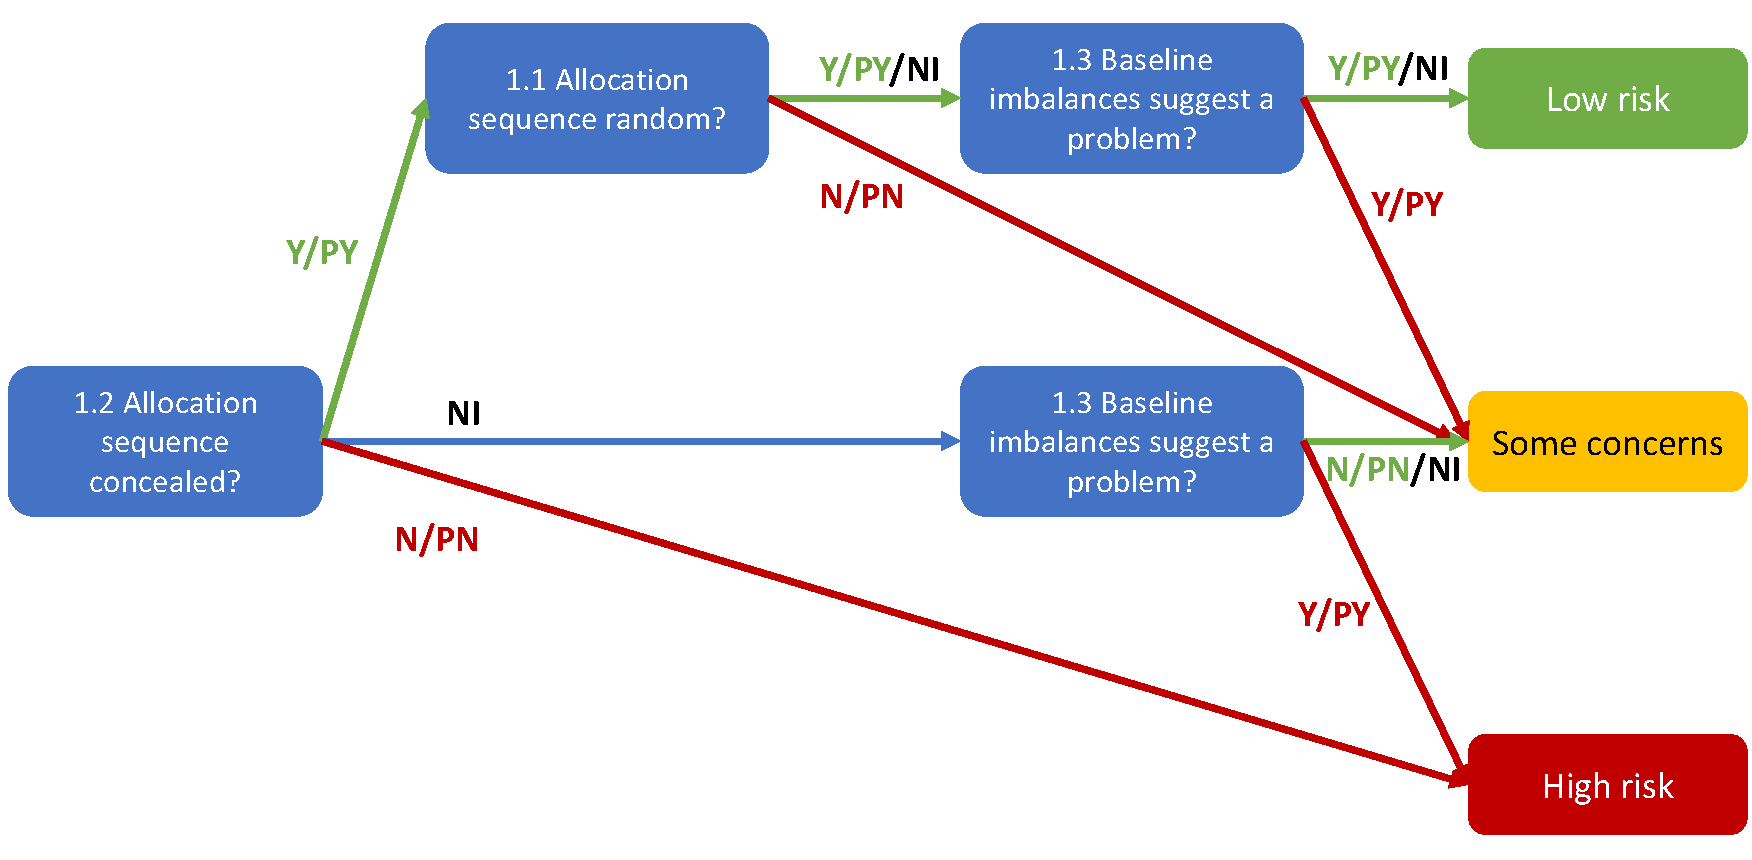
\includegraphics[width=0.80\columnwidth]{figures/flowchart.pdf}
    \caption{Algorithm for suggested judgement of risk of bias arising from the randomization process. The figure is recreated from the revised Cochrane's risk of bias tool (RoB 2).~\cite{sterne2019rob}}
    \label{fig:flowchart}
\end{figure}
%
%
%

%
%
%
\subsection{Expert team}
\label{experts}
%
As mentioned earlier, RoB annotation is a complex task that requires specialized expertise.
It is cognitively demanding due to the need to carefully go through the entire full-text of RCTs and identify 22 different bias categories for annotation.
This level of complexity would not be manageable for annotators without expertise in the field.
Our annotation team consisted of two researchers specializing in RoB assessment in physiotherapy and rehabilitation domains, including an epidemiology researcher and an assistant professor in physiotherapy.
With a substantial background in both physiotherapy, advanced statistical methods and experience writing SRs, both experts possessed a deep understanding of the complexities involved in bias assessment.
Two additional physiotherapy experts, a post doctoral researcher and a senior PhD student, were a part of developing the visual annotation guidelines.
Two additional researchers with expertise in natural language processing (NLP) were involved, a computational linguistics professor and a PhD student in computer science.
Their inclusion was important because the guidelines and placards they helped create will be utilized to annotate a text corpus, serving as a benchmark for RoB text span extraction.
%
%
%
\subsection{Data collection}
\label{data}
%
Savović~\textit{et al.} categorized outcome measures as mortality, other objective outcome, and subjective outcome and estimated the associations of bias judgments with intervention effect estimates~\cite{savovic2018association}.
Trials assessing subjective outcomes are more prone to bias, therefore, had we used only one outcome type, we would have limited label types for different risk classes~\cite{page2016empirical}.
In context of RCTs, subjective outcomes are measurements that rely on individuals' perceptions, opinions, or feelings about their own health or well-being.
These outcomes are typically self-reported by the participants in the trial and can be influenced by factors such as  placebo effects, patient expectations, interpretation, and psychological factors.
For example, in a study on rheumatoid arthritis, subjective outcome measures included patient-reported pain ratings~\cite{vollert2020assessment}.
Objective outcomes are measurements that are independent of individual opinions or perceptions and are based on observable and measurable data.
These outcomes are typically collected by trained assessors or through laboratory tests, imaging studies, or other objective methods.
For instance, in a study on peripheral artery disease, objective outcome measures included angiography and molecular imaging to evaluate the effectiveness of cell therapy~\cite{grimaldi2016imaging}.
Mortality outcomes refer to the occurrence of death during the course of the trial.
To ensure these different outcome types are represented in the corpus, we included 17, 17 and 7 RCTs addressing objective, subjective and mortality primary outcomes.
The epidemiology researcher from our team created this 41 RCTs dataset from the domain of physiotherapy and rehabilitation.
PDFs of the full-text RCTs were extracted and each article was collated with its trial protocol from wherever available.
Corpus details are in the Supplementary material.
%
%
%
\subsection{Visual Placards Development}
\label{guidelines}
%
RoB 2 tool consist of extensive and step-by-step set of instructions to answer signaling questions and even though RoB 2 guidelines are widely used for bias assessment, there have been some research on their reliability.
This reliability concern has been extensively investigated by Minozzi \textit{et al.}. 
They formulated specific instructions on how to approach and answer the signaling questions of RoB 2.
These instructions, referred to as the Instruction Document (ID), address the subjectivity present in the RoB 2 guidelines and provide clear guidance for the assessment process.
Subjectivity in assessment could potentially result in different evaluators coming to disparate conclusions when analyzing the same trial.
Before implementing the ID, the agreement among four expert RoB assessors was zero, but it improved after adopting the ID.
Several other papers explored subjectivity and reliability of the Cochrane RoB 1.0 and 2 tools~\cite{minozzi2022reliability,da2017effect,loef2022interrater,minozzi2020revised}.
With this in mind, we developed precise and clear text annotation instructions using the RoB 2 tool with an aim to maintain the consistency and reliability among annotators.
Working closely with our team of experts, we formatted these instructions into visual instructional placards.
Each placard takes the form of a flowchart and provides instructions for annotating RCT text to answer a SQ.
The flowchart also provides instructions on labelling the annotated text with risk judgment.
The RoB 2 tool SQs are broadly factual but leave room for subjective judgements and our visual placards aim to facilitate judgements about the risk of bias.
%
%
%
\subsection{Annotation}
\label{annotation}
%
%
%
%
\begin{figure}[htb]
    \centering
    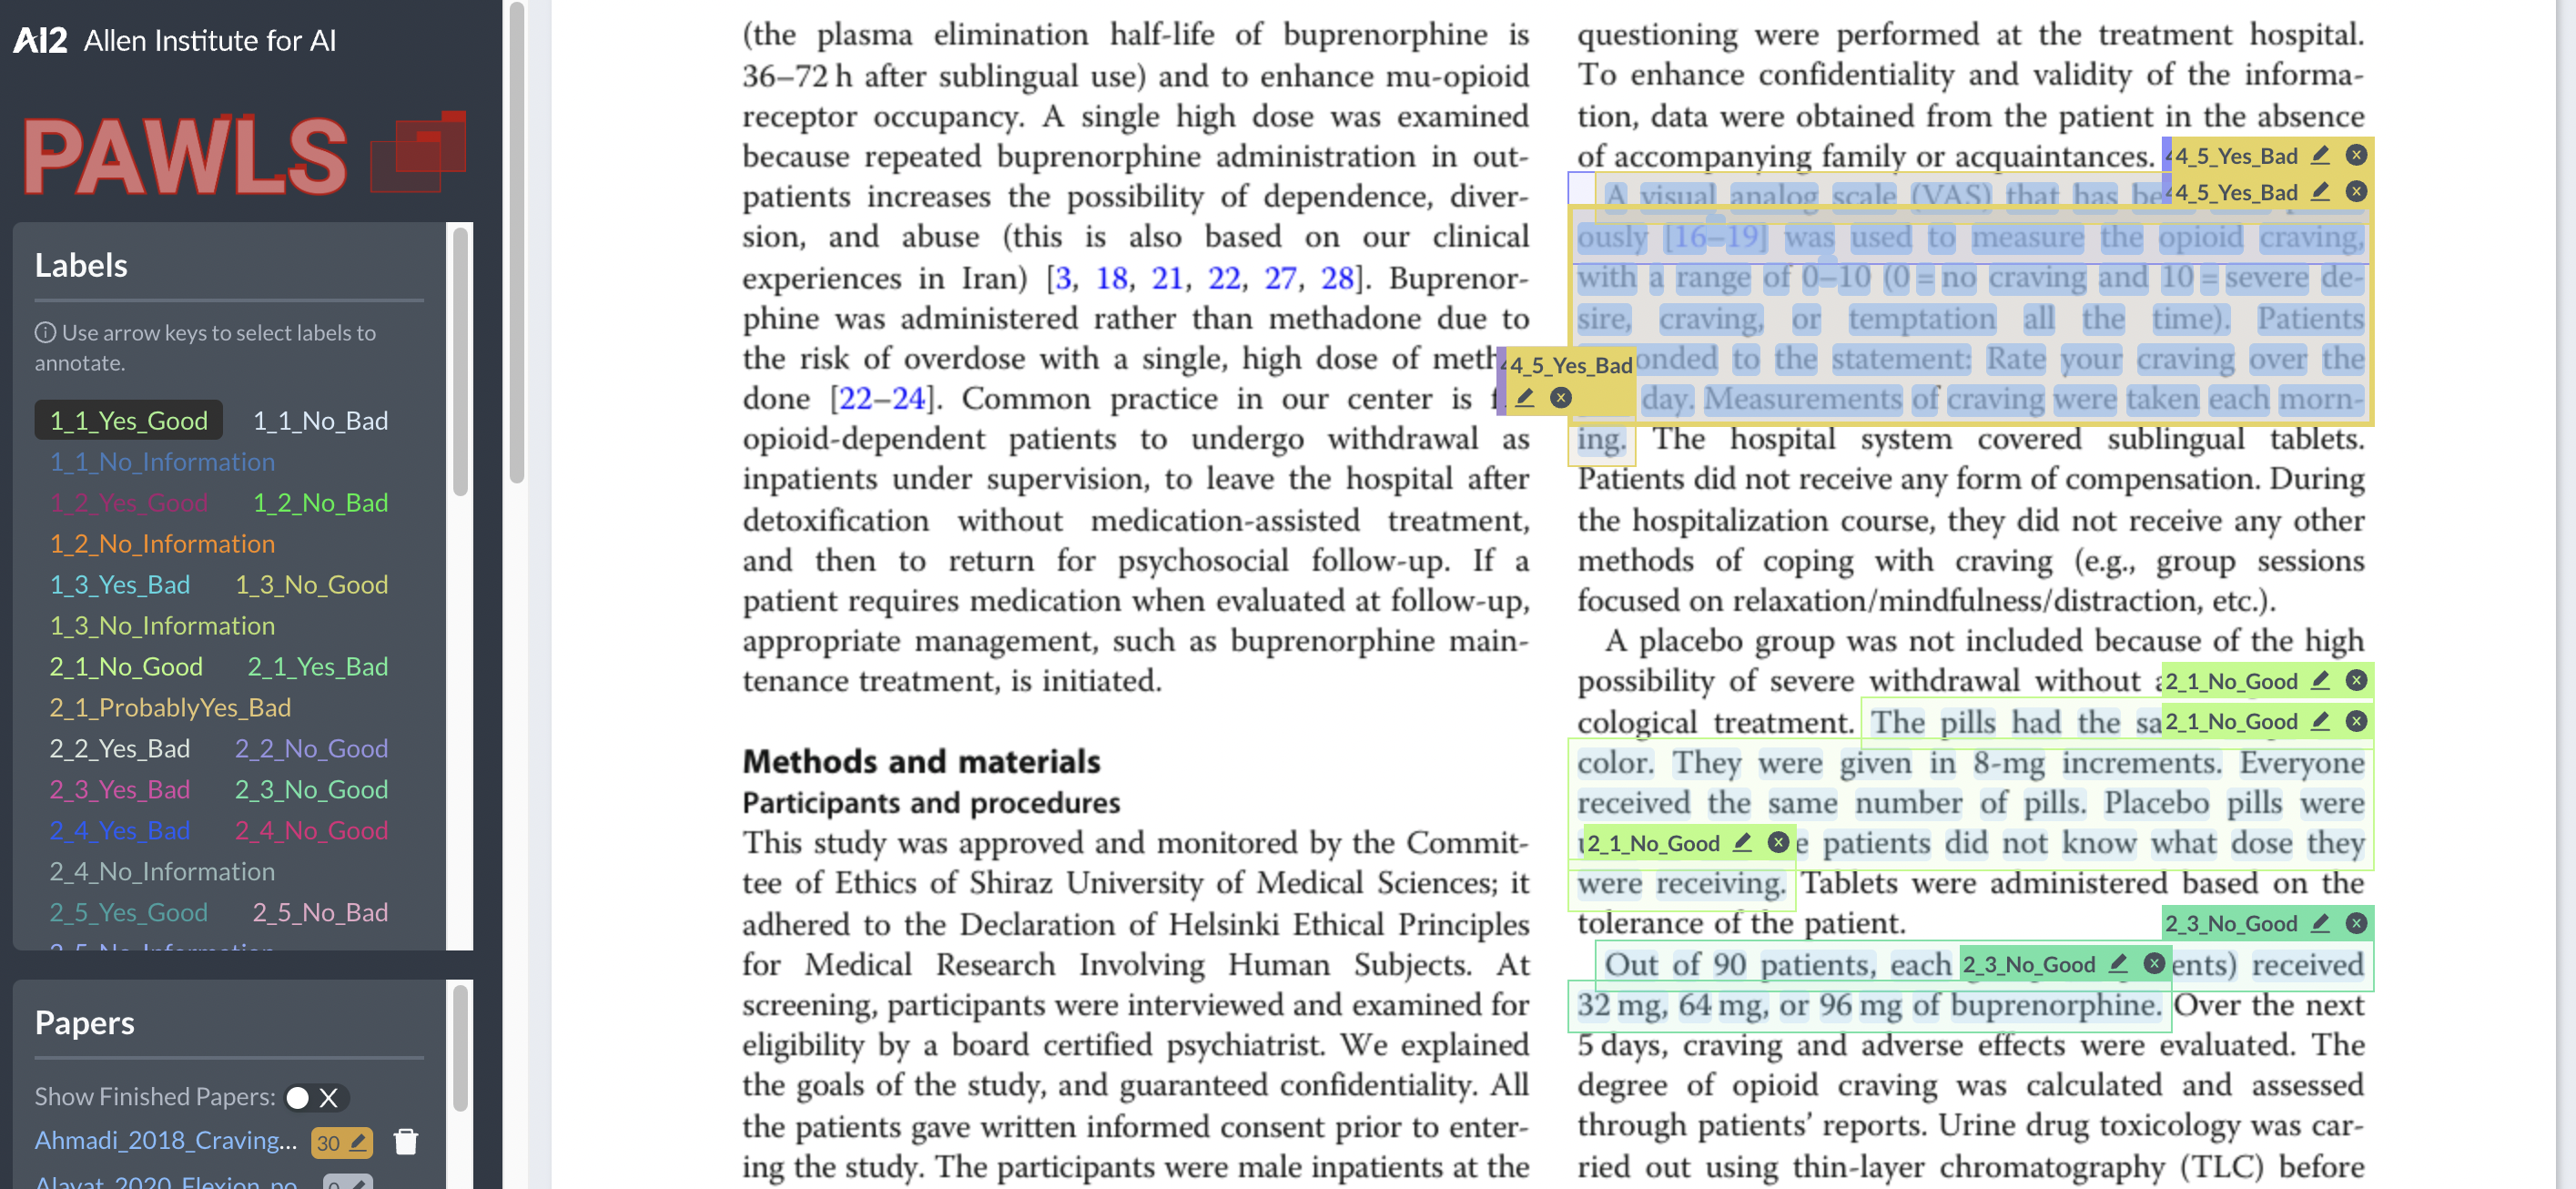
\includegraphics[width=0.80\columnwidth]{figures/pawls_layout.png}
    \caption{A screenshot of PAWLS interface with an example PDF and RoB annotations.}
    \label{fig:pawls}
\end{figure}
%
%
%
For every SQ, the annotators were guided to use the complete RoB 2 guidance document along with visual placards that were developed.
They followed these instructions meticulously, going through each placard's signaling question one by one.
The provided instructions directed the annotators to read specific sections of full-text RCT that needed annotation.
Their task involved identifying and highlighting relevant text related to answering the signaling question.


Tagtog~\footnote{\url{https://www.tagtog.net/}}, a commercial text annotation web application, allows for annotating PDF (Portable Document Format) documents, was used for the annotation~\cite{cejuela2014tagtog}.
Out of the 60 documents, 9 were doubly annotated by two experienced annotators (a epidemiology researcher and an assistant professor) to calculate inter-annotator agreement (IAA) over these documents and the rest were singly annotated by the epidemiology researcher.
After double annotation, we performed conflict resolution to address conflicting annotations, which helped us further calibrate the visual placards.
The conflict resolution was followed by annotating 51 additional RCTs.


After the annotation of 9 doubly-annotated RCTs, we had to stop using tagtog for certain reasons and switched to the PAWLS~\footnote{\url{https://pawls.apps.allenai.org/}} annotation tool, which allows users to annotate PDFs for free~\cite{neumann2021pawls}.
We chose to annotate PDFs rather than plain text because RCT PDFs have a visual format that will be lost upon converting to text. 
For example the structure pertaining to sections and subsections, tables, and figures makes the annotation task quicker for the annotators and increases annotation quality.
Post annotation, the feedback was taken from both the annotators details of which could be found in the supplementary material. %TODO Anjani: Prepare the supplementary material 
%
%
%
\subsection{Inter-Annotator Agreement}
\label{method:iaa}
%
We report IAA at two levels checking whether the annotators agree on the text spans to answer SQs using the pairwise F1 measure.
F1-measure disregards out-of-the-span tokens (unannotated tokens) during agreement calculation and is an ideal measure of annotation reliability for the token-level annotation tasks.
It measures the F1 score for each pair of annotators, treating one annotator's labels as the ``true'' labels and the other annotator's labels as the ``predicted'' labels~\cite{deleger2012building,brandsen2020creating}.
We also check how strongly the annotators agree on the risk judgment for each SQ using prevalence and bias adjusted kappa (PABAK) $\kappa_{pabak}$ and compare it with raw percent agreement.
PABAK $\kappa_{pabak}$ is the standard annotation reliability measure for many classification annotation tasks and is suitable to measure reliability at the risk judgment level.
$\kappa_{pabak}$ is an extension of Cohen's Kappa $\kappa$ that takes into account prevalence and bias in the agreement.
We interpret both IAA measures as shown in the Table~\ref{tab:iaa_interpret}~\cite{mchugh2012interrater,cohen1960coefficient,byrt1993bias,landis1977measurement}.
%
%
%
\begin{center}
 \begin{table}[htb]
   \caption{The table details interpretation of pairwise F1-measure (Left), $\kappa_{pabak}$ (Middle) and observed or raw agreement (Left)}\label{tab:iaa_interpret}
 \centering
    \begin{tabular}{lr|lr|lr}
    \toprule[1.0pt]
    \multicolumn{2}{c|}{F1-measure} & \multicolumn{2}{c|}{$\kappa_{pabak}$}& \multicolumn{2}{c}{Raw Agreement}  \\ 
    interpretation & range & interpretation & range & interpretation & range \\ 
    \midrule[1.0pt]
        Poor & 0-0.99 &  No agreement& $\leq$ 0 & None & 0 \\ 
        Slight & 1 - 20.99 &  None to slight agreement & 0-0.20 & Very low & 1-10\% \\ 
        Fair & 21 - 40.99 &  Minimal & 0.21-0.39 & Low & 11-30\% \\ 
        Good & 41 - 60.99 & Weak & 0.40-0.59 & Moderate & 31-50\% \\ 
        Substantial & 61 - 80.99 & Moderate & 0.60-0.79 & High & 51-70\% \\ 
        Almost perfect & 81 - 99.99 & Strong & 0.80-0.90 & Very high & 71-90\% \\ 
        Perfect & 100 & Almost Perfect & $\geq$ 0.90 & Perfect & $>$90\% \\ 
         & & Perfect & 1.0 \\ 
    \bottomrule[1.0pt]
    \end{tabular}
 \end{table}   
\end{center}
%
%
%
\subsection{LLM evaluation}
\label{method:llm}
%
Our annotation guidelines and annotations were adapted for benchmarking supervised machine learning approaches and not LLMs.
So even though we were annotating PDFs, we had to restrict a lot of annotations based on the assumption that PDF will be converted into text via OCR (optical character recognition) losing its structure of tables and figures, which anyway a classical ML model could not use without extensive modifications~\cite{li2019figure,li2023uttsr}.
Recent advancements with LLMs that encode vast amounts of knowledge offers a better alternative made us rethink the evaluation.
The bar for clinical applications is high and it is imperative to evaluate LLMs for the more challenging clinical tasks like RoB text span extraction~\cite{singhal2023large}.
The tools like ChatPDF~\footnote{\url{https://www.chatpdf.com/}} allow direct interaction between LLMs and PDFs, negating the clumsy PDF to text conversion.
Therefore, we consider it essential to evaluate LLMs instead of forcefully adapting the evaluation to a classical ML problem.
We formulated the task as a zero-shot RoB text span extraction task.
This was to gauge whether an LLM encodes knowledge related to assessing trial biases.
We will use simple prompt constructs of the structure ``Answer the \{\textit{SQ}\} + Action item to extract sentence supporting the answer''.
Consider the following example.

\begin{quote}
\itshape Example prompt: Question 4.3 Were outcome assessors aware of the intervention received by study participants? Provide an answer and extract the supporting sentences that you write your answer based on. Extract the sentences in JSON~\footnote{JSON = JavaScript Object Notation}.
\end{quote}

The prompt serves two purposes for evaluating LLMs for correctness.
LLM is prompted to 1) answering the SQ with a response option (risk judgment), and 2) extract the text evidence to support their answer.
When answering a question, ChatPDF finds the most relevant paragraphs from the PDF and uses the ChatGPT API from OpenAI to generate an answer~\footnote{ChatPDF employs GPT (Generative Pretrained Transformer) 3.5.}.
LLM is required to do the same task as human annotators and will be evaluated on the basis of correctness of the answer.
If LLM answer corresponds to response option selected by the expert annotator, it is considered a correct answer for that SQ. 
If the text extracted by LLMs as evidence for answering the SQ fuzzy matches the text selected by the expert annotator, it is considered a correct answer.
Both of these skills will be evaluated using a raw or observed agreement metrics $P_{O} (Extraction)$  for measuring agreement over extraction and $P_{O} (Response)$ for measuring agreement over response judgments and interpreted as per Table~\ref{tab:iaa_interpret}. 
Observed agreement is essentially the number of documents for a RoB SQ where LLM responses align with those of the human expert, divided by the total number of documents assessed~\cite{artstein2017inter}.
In several instances, there was no information found by the expert annotator from the RCT to answer a question. 
For such instances, if ChatPDF correctly identifies the absence of relevant information to answer a question, it is considered a correct response.
It's important to highlight that the evaluation framework is designed solely to measure the agreement of the answers between ChatPDF and the expert.
LLM evaluation was manually conducted by a bias assessment expert and an NLP expert for 10 out of the 41 RCTs.
%
%
%
\section{Results}
\label{sec:results}
%
This section outlines the visual placards, annotated dataset, reports the IAA findings, and the outcomes of the LLM evaluation.
%
%
%
\subsection{Visual Placards}
\label{result:placards}
%
%
%
%
\begin{figure}
    \centering
    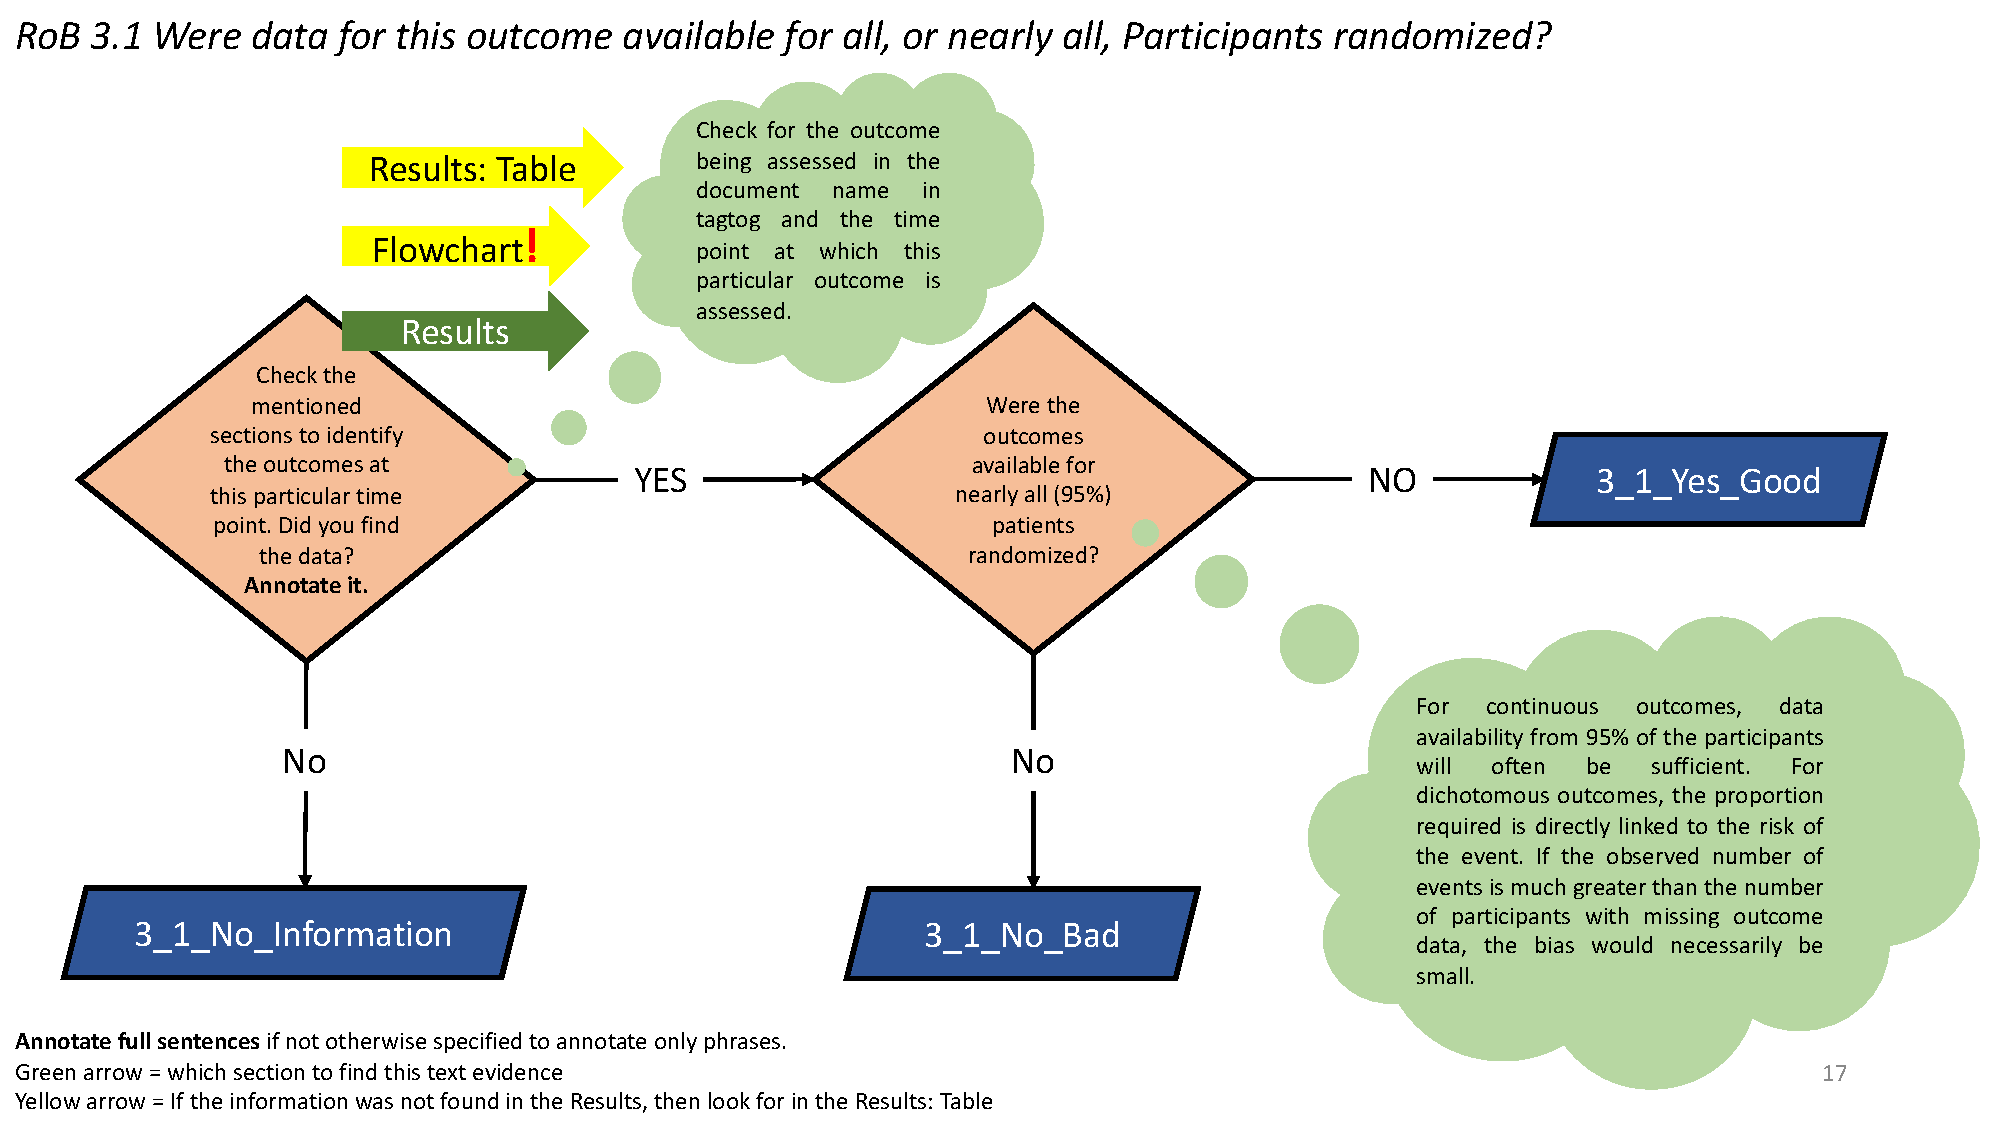
\includegraphics[width=0.80\columnwidth]{figures/placard_3_1.pdf}
    \caption{Sample annotation instruction placard for the SQ 3.1 designed and adapted using RoB 2 tool.}
    \label{fig:placard}
\end{figure}
%
%
%
A total of 27 placards were developed to address the 22 signalling questions in RoB 2 tool. 
Details of the annotation guidelines and visual placards are available in the Supplementary material.
Figure~\ref{fig:placard} presents an example placard for annotating SQ 3.1 (``Were data for this outcome available for all, or nearly all participants randomized?'') which assesses the completeness of outcome data in an RCT.
This question assesses whether data for the specific outcome of interest were collected and available for analysis for a high proportion of initially randomized participants.
Missing data can compromise statistical power and treatment effect estimates. 
The first diamond on the placard instructs annotators to check the Results section (first priority) and the flowchart (second priority) to identify outcome data at the specified time point.
If outcomes data were available for at least 95\% of participants, annotators mark relevant text descriptions as ``3.1 Yes Good'' indicating a low bias.
If data were available for less than 95\%, they mark it as ``3.1 No Bad'' indicating a high bias.
Lack of information will lead to automatically assuming a ``No Information'' label.
The yellow arrow on the first diamond suggests checking the Results section first; if not found, annotators should look in the Results section table.
If still not found, annotators are instructed to check the flowchart caption, marked with a red exclamation as a last resort.
%
%
%
\subsection{The corpus: RoBuster}
\label{subsec:corpus}
%
We provide key statistical information about the annotations in RoBuster in this section.
The histogram in Figure \ref{fig:ann_counts} shows a visual representation of the absolute counts of annotations (tokens) for each of the RoB SQs.
SQ 1.3 had disproportionately higher number of annotated tokens, while for all other SQs, the number of annotated tokens remained consistently below 2000 across the entire corpus.
The only exception to this trend was for SQ 3.1 which had slightly more than 2000 annotated tokens.
SQ 2.4 ("Were these deviations likely to have affected the outcome?") had only 25 annotated tokens.


Table~\ref{table:stats} lists down essential information on the absolute and average annotation lengths for each RoB SQ along with the total number of documents the annotations were identified from.
Annotations for the ``randomization'' risk domain 1 were found in an average of 35 of the 41 documents, while annotation related to answering the other risk questions was available only in a small subset of the total annotated RCTs, as also depicted in Figure~\ref{fig:rob_information} which shows the distribution of risk judgments across RoBuster.
The figure highlights that, for most SQs, no information was available (indicated by yellow bars) for answering the SQs and making the risk judgment.
Notably, SQs 2.2, 2.6, 3.1, 4.3, and 4.4 stood out as exceptions, with information available in more than 50\% of the annotated documents.
In cases where information was available, bias tended to be low, as indicated by the prevalence of green bars with an exception for the SQs 2.2, 3.1, 4.3, and 4.4, where bias was high, as indicated by the prevalence of red bars.
Check the Supplementary material for the references of all the studies in RoBuster.
%
%
%
\begin{figure}[htb]
    \centering
    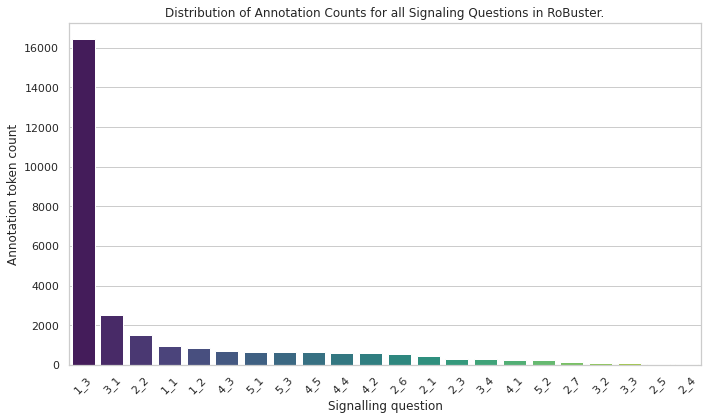
\includegraphics[width=0.90\columnwidth]{figures/annot_counts.png}
    \caption{Total number of token annotations for each RoB SQ.}
    \label{fig:ann_counts}
\end{figure}
%
%
%

%
%
%
\begin{table}[htb]
    \centering
    \caption{General statistics for the annotated corpus: This table provides an overview of the annotated corpus, including the total number of annotated tokens, the average length of token sequences, and the number of documents in which annotations were identified, out of a total of 41 annotated documents.}
    \label{table:stats}
    \begin{tabular}{crrr}
    \toprule[1.0pt]
        SQ & Total tokens & Average length & Total documents \\
    \midrule[1.0pt]
        \multicolumn{4}{c}{Domain 1: Biases arising from the randomization process} \\
        \hline
        RoB1.1 & 960 & 32 & 30 \\
        RoB1.2 & 838 & 24.65 & 34 \\
        RoB1.3 & 16446 & 411.15 & 40 \\
        \hline
        \multicolumn{4}{c}{Domain 2: Biases due to deviations from intended interventions} \\
        \hline
        RoB2.1 & 455 & 32.5 & 14 \\
        RoB2.2 & 1502 & 55.63 & 27 \\
        RoB2.3 & 282 & 56.4 & 5 \\
        RoB2.4 & 25 & 25 & 1 \\
        RoB2.5 & 58 & 29 & 2 \\
        RoB2.6 & 544 & 20.92 & 26 \\
        RoB2.7 & 126 & 25.2 & 5 \\
        \hline
        \multicolumn{4}{c}{Domain 3: Bias due to missing outcome data} \\
        \hline
        RoB3.1 & 2529 & 74.38 & 34 \\
        RoB3.2 & 103 & 34.33 & 3 \\
        RoB3.3 & 75 & 15 & 5 \\
        RoB3.4 & 276 & 21.23 & 13 \\
        \hline
        \multicolumn{4}{c}{Domain 4: Bias in the measurement of the outcome} \\
        \hline
        RoB4.1 & 240 & 24 & 10 \\
        RoB4.2 & 572 & 33.65 & 17 \\
        RoB4.3 & 698 & 30.35 & 23 \\
        RoB4.4 & 585 & 27.86 & 21 \\
        RoB4.5 & 622 & 41.47 & 15 \\
        \hline
        \multicolumn{4}{c}{Domain 5: Bias in the selection of the reported result} \\
        \hline
        RoB5.1 & 628 & 69.78 & 9 \\
        RoB5.2 & 235 & 19.58 & 12 \\
        RoB5.3 & 628 & 89.71 & 7 \\
    \bottomrule[1.0pt]
    \end{tabular}
\end{table}
%
%
%

%
%
%
\begin{figure}[htb]
    \centering
    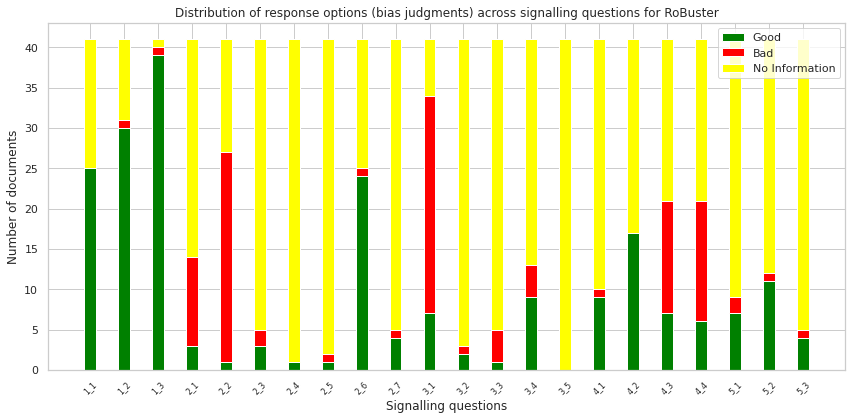
\includegraphics[width=0.90\columnwidth]{figures/bias_chart.png}
    \caption{Distribution of bias judgment across RoB SQs in RoBuster.}
    \label{fig:rob_information}
\end{figure}
%
%
%

%
%
%
\subsection{Inter-annotator agreement}
\label{result:iaa}
%
Table~\ref{tab:IAA_sq} illustrates the levels of F1-measure (inter-annotator agreement) between the two annotators, both before and after the development of the visual placards.
The F1-measure before and after the guideline improvement were calculated on a different set of documents.
The average overall F1 agreement across the corpus exhibited a modest 10.87\% agreement before the introduction of visual placards.
Following their implementation, this agreement increased significantly by 17.14 percent points, reaching a fair 28.01\%.
The agreement for the ``randomization'' domain 1 doubled from a poor (F1 31.72 IAA) to a substantial (F1 63.30 IAA).
For the ``deviations from intended interventions'' domain 2, the agreement increased from a slight (F1 (F1 12.76 IAA) to fair (F1 27.02 IAA).
In the case of the ``missing outcomes'' domain 3, the agreement rose from (F1 5.89 IAA) to (F1 9.92 IAA), although it remained within the slight agreement category. 
For the ``missing outcome measurement'' domain 4 the agreement increased from (F1 4.072 IAA) to (F1 17.29 IAA).
The agreement before the placard development was none and it increased to slight (F1 16.49 IAA) for the ``selection of reported results'' domain 5.


Improvements in agreement were observed at individual SQs level too, with considerable gains exceeding 50\% points for signaling questions 1.3, 2.1, 4.1, and 4.4.
The F1-measure between the two reference annotators for a total of 11 out of 22 questions remained zero both before and after the guideline development.
For two SQs, 4.4 and 5.2, the guideline improvement raised it from zero to 56.25 and 49.49 respectively.
However, for SQs 2.3 and 2.7, the agreement experienced a modest decline of 5.42 and 6.52, reaching zero after the guideline development.
For the SQ 1.2, the agreement dropped by 6.28 IAA points making it a drop in agreement for three SQs.
Inferring from the table~\ref{tab:iaa_interpret} and table~\ref{tab:IAA_sq}, annotators for 11 of the 22 SQs had a poor agreement, three of the 22 questions had a fair agreement, four out of the 22 questions had a good agreement and two out of the 22 questions had a substantial agreement while only two of the 22 questions had an almost perfect agreement of beyond 81 IAA points.
As expected, none of the SQ annotations had a perfect F1-measure.
%
%
%
\begin{table}[htb]
    \caption{The table displays the F1-Measure at the text span annotation level before and after the development of visual placards. The change in F1-Measure is presented in terms of absolute IAA points.}
    \label{tab:IAA_sq}
    \centering
    \begin{tabular}{crrr}
    \toprule[1.0pt]
         & \multicolumn{2}{c}{F1-measure IAA} & \\
        SQ & before guideline improvement & after guidelines improvement & change \\
    \midrule[1.0pt]
        \multicolumn{4}{c}{Domain 1: Biases arising from the randomization process} \\
        \hline
        RoB 1.1 & 24.44 & 55.02 & +30.58 \\ 
        RoB 1.2 & 50.28 & 44 & -6.28 \\ 
        RoB 1.3 & 20.44 & 90.9 & +70.46 \\
        \hline
        \multicolumn{4}{c}{Domain 2: Biases due to deviations from intended interventions} \\
        \hline
        RoB 2.1 & 1.34 & 67.26 & +65.92 \\ 
        RoB 2.2 & 7.23 & 38.66 & +31.43 \\ 
        RoB 2.3 & 5.42 & 0 & -5.42 \\ 
        RoB 2.4 & - & 0 & 0 \\ 
        RoB 2.5 & 0 & 0 & 0 \\ 
        RoB 2.6 & 68.85 & 83.25 & +14.4 \\ 
        RoB 2.7 & 6.52 & 0 & -6.52 \\ 
        \hline
        \multicolumn{4}{c}{Domain 3: Bias due to missing outcome data} \\
        \hline
        RoB 3.1 & 23.57 & 39.68 & +16.11 \\ 
        RoB 3.2 & 0 & 0 & 0 \\ 
        RoB 3.3 & 0 & 0 & 0 \\ 
        RoB 3.4 & 0 & 0 & 0 \\ 
        \hline
        \multicolumn{4}{c}{Domain 4: Bias in the measurement of the outcome} \\
        \hline
        RoB 4.1 & 6.51 & 61.71 & +55.2 \\ 
        RoB 4.2 & 0 & 0 & 0 \\ 
        RoB 4.3 & 13.85 & 30.21 & +16.36 \\ 
        RoB 4.4 & 0 & 56.25 & +56.25 \\ 
        RoB 4.5 & 0 & 0 & 0 \\ 
        \hline
        \multicolumn{4}{c}{Domain 5: Bias in the selection of the reported result} \\
        \hline
        RoB 5.1 & 0 & 0 & 0 \\ 
        RoB 5.2 & 0 & 49.49 & +49.49 \\ 
        RoB 5.3 & 0 & 0 & 0 \\
    \bottomrule[1.0pt]
    \end{tabular}
\end{table}
%
%
%

We present the prevalence and bias adjusted kappa $\kappa_{pabak}$ agreement, raw agreement and the percentage of $\kappa_{pabak}$ agreements
that stemmed from the ``No Information'' judgments in Table~\ref{tab:IAA_response}.
To recall $\kappa_{pabak}$ measures agreement at the SQ risk judgment level~\cite{mchugh2012interrater}.
The overall $\kappa_{pabak}$ agreement between the annotators stand at a weak IAA of 0.41181 IAA.
The average agreement for ``randomization'' domain 1 was a moderate 0.629 IAA.
For the ``deviations due to intended interventions'' (domain 2), there was a moderate agreement of 0.64 IAA and for the ``due to missing outcome data'' (domain 3) there was a minimal agreement of 0.388 IAA.
The last two domain 4 and 5 ``measurement of the outcome'' and ``selection of the reported result'' had agreements 0.166 IAA and 0.092 IAA interpreted slight and no agreement.



The highest agreement of 1.0 is observed for SQ 2.6.
It is, however, important to note that more than half of this agreement arises from the assumed ``No Information'' judgments for 2.6.
For the remaining SQs, we do not find any instances of either almost perfect or strong agreement.
Agreements for SQs 1.1, 2.1, 2.5, 3.1, and 4.3 fall within the moderate agreement category ranging from 0.60 to 0.80 IAA.
Amongst these SQs, only for the SQ 1.1, 2.1, 3.1 and 4.3 has no substantial agreement originating from the ``No Information'' judgments.
In contrast, two of the 22 signaling questions (4.2 and 5.1) exhibit agreement worse than what would be expected by chance.
The bias questions 3.3 and 4.5 show zero $\kappa_{pabak}$ agreement.


%
%
%
\begin{table}[]
    \caption{Prevalence and Bias adjusted Kappa $\kappa_{pabak}$ and raw agreement between annotator pairs for agreement at the risk judgment level for each SQ.}
    \label{tab:IAA_response}
    \begin{tabular}{crrr}
    \toprule[1.0pt]
        SQ & $\kappa_{pabak}$ agreement & Raw agreement & Contribution from ``No Information'' \\
    \midrule[1.0pt]
        \multicolumn{4}{c}{Domain 1: Biases arising from the randomization process} \\
        \hline
        RoB 1.1 & 0.8333 & 88.90\% & 22.22\% \\
        RoB 1.2 & 0.5 & 66.70\% & 33.33\% \\
        RoB 1.3 & 0.5556 & 77.80\% & 11.11\% \\
        \hline 
        \multicolumn{4}{c}{Domain 2: Biases due to deviations from intended interventions} \\
        \hline
        RoB 2.1 & 0.7037 & 77.80\% & 5.56\% \\
        RoB 2.2 & 0.5 & 66.70\% & 38.89\% \\
        RoB 2.3 & 0.5 & 66.70\% & 77.78\% \\
        RoB 2.4 & 0.5556 & 77.80\% & 88.89\% \\
        RoB 2.5 & 0.6667 & 77.80\% & 83.33\% \\
        RoB 2.6 & 1 & 100.00\% & 55.56\% \\
        RoB 2.7 & 0.5556 & 77.80\% & 77.78\% \\
        \hline
        \multicolumn{4}{c}{Domain 3: Bias due to missing outcome data} \\
        \hline
        RoB 3.1 & 0.8333 & 88.90\% & 11.11\% \\
        RoB 3.2 & - & 100.00\% & 100.00\% \\
        RoB 3.3 & 0 & 33.30\% & 55.56\% \\
        RoB 3.4 & 0.3333 & 55.60\% & 33.33\% \\
        \hline
        \multicolumn{4}{c}{Domain 4: Bias in the measurement of the outcome} \\
        \hline
        RoB 4.1 & 0.5556 & 77.80\% & 11.11\% \\
        RoB 4.2 & -0.5556 & 22.20\% & 38.89\% \\
        RoB 4.3 & 0.6667 & 77.80\% & 27.78\% \\
        RoB 4.4 & 0.1667 & 44.40\% & 22.22\% \\
        RoB 4.5 & 0 & 33.30\% & 66.67\% \\
        \hline
        \multicolumn{4}{c}{Domain 5: Bias in the selection of the reported result} \\
        \hline
        RoB 5.1 & -0.5556 & 22.20\% & 61.11\% \\
        RoB 5.2 & 0.5 & 66.70\% & 22.22\% \\
        RoB 5.3 & 0.3333 & 55.60\% & 72.22\% \\
    \bottomrule[1.0pt]
    \end{tabular}
\end{table}

%
%
%
\subsection{LLM evaluation}
%
In Table~\ref{table:LLM_eval}, we present the observed or raw agreement ($P_{O}$) between LLM and expert assessments in extracting and responding to SQ over a subset (n=10) of RoBuster~\ref{method:llm}. 
The evaluation was conducted on four RCTs reporting objective outcome, three RCTs evaluating subjective outcome and the rest three RCTs reporting mortality outcome.
For the first risk domain, ChatGPT had high $P_{O} (Extraction)$ and $P_{O} (Response)$ agreements (66.6\% and 55.3\% IAA respectively) with experts and none of these agreements came from ``No Information'' responses indicating a good availability of information for bias assessment. 
Notably, for individual SQs within domain 1, the $P_{O} (Extraction)$ was greater than $P_{O} (Response)$.
The observed agreements for the the second domain are even higher 64.28\% and 60\% respectively, but 40\% of these agreements emanate from ``No Information'' responses suggesting lower availability of information. 
Domain 3 exhibited a moderate average observed agreement of 47.5\% for both $P_{O} (Response)$ and $P_{O} (Extraction)$ , while Domain 4 demonstrated a lower observed agreement of 28\% and 26\% for response and extraction, respectively.
\textcolor{blue}{The results for risk domain 5 remain.}
Details about the RCTs used for LLM evaluation are in the Supplementary material.
%
%
%
\begin{table}[htb]
    \caption{LLM accuracy}
    \label{table:LLM_eval}
    \centering
    \begin{tabular}{crrr}
    \toprule[1.0pt]
     & \multicolumn{2}{c}{Observed Agreement $P_{O}$} \\
        SQ & $P_{O} (Extraction)$ & $P_{O} (Response)$ & ``No Information'' \\ 
    \midrule[1.0pt]
        \multicolumn{4}{c}{Domain 1: Biases arising from the randomization process} \\
        \hline
        RoB 1.1 & 90\% & 70\% & 0\% \\ 
        RoB 1.2 & 70\% & 60\% & 0\% \\ 
        RoB 1.3 & 40\% & 30\% & 0\% \\ 
        \hline
        \multicolumn{4}{c}{Domain 2: Biases due to deviations from intended interventions} \\
        \hline
        RoB 2.1 & 50\% & 40\% & 0\% \\
        RoB 2.2 & 30\% & 30\% & 10\% \\ 
        RoB 2.3 & 60\% & 60\% & 50\% \\ 
        RoB 2.4 & 90\% & 90\% & 100\% \\ 
        RoB 2.5 & 90\% & 90\% & 100\% \\ 
        RoB 2.6 & 80\% & 50\% & 10\% \\ 
        RoB 2.7 & 50\% & 60\% & 40\% \\
        \hline
        \multicolumn{4}{c}{Domain 3: Bias due to missing outcome data} \\
        \hline
        RoB 3.1 & 30\% & 40\% & 0\% \\ 
        RoB 3.2 & 60\% & 40\% & 40\% \\ 
        RoB 3.3 & 30\% & 30\% & 30\% \\ 
        RoB 3.4 & 70\% & 80\% & 70\% \\ 
        \hline
        \multicolumn{4}{c}{Domain 4: Bias in the measurement of the outcome} \\
        \hline
        RoB 4.1 & 40\% & 30\% & 10\% \\ 
        RoB 4.2 & 40\% & 30\% & 20\% \\ 
        RoB 4.3 & 10\% & 10\% & 10\% \\ 
        RoB 4.4 & 10\% & 20\% & 10\% \\ 
        RoB 4.5 & 40\% & 40\% & 40\% \\
        \hline
        \multicolumn{4}{c}{Domain 5: Bias in the selection of the reported result} \\
        \hline
        RoB 5.1 & & & \\ 
        RoB 5.2 & & & \\ 
        RoB 5.3 & & & \\
    \bottomrule[1.0pt]
    \end{tabular}
\end{table}
%
%
%
\section{Discussion}
\label{sec:discussion}
%
\subsection{Visual Placards}
\label{disc:placards}
%
As per~\cite{dhrangadhariya2023first}, there were two reasons causing a low F1 IAA for annotating text span to answer a SQ.
One reason was a lack of instructions whether the annotators should annotate a phrase, a sentence or sentences.
While some annotators might annotate an entire paragraph as text evidence to answer a SQ, others might focus on the most informative portion of the text.
To address this, our placards provide clear guidance on whether annotators should annotate a phrase, a sentence, or a combination of sentences.
Another common reason for a low F1 was when annotators correctly addressed a bias SQ but annotated evidence from different parts of the full text leading to no or low agreement. 
To tackle this, our placards restrict annotations for a question to a specific part of the text for specific SQs, such as the Methods section, Results section, Flowchart in the Methods section, etc.



The visual placards addressed various facets of RoB 2 subjectivity and also when dealing with situations lacking information for risk judgment annotation.
In one trial document annotation, both annotators selected the phrase ``71 allocated routine services, 67 allocated intervention service, 69 assessed at 8 weeks, 64 assessed at 8 weeks'' from the PRISMA flowchart to answer signaling question 3.1~\cite{gilbertson2000domiciliary}.
However, one annotator responded with ``Yes'' while the other chose ``No''.
This question asks whether outcome data were available for all or nearly all participants randomized, but it doesn't specify the exact cutoff for participant dropouts that increase the risk.
Therefore, annotators make subjective judgments based on their experience regarding what percentage of participant dropout is considered valid.
To address this subjectivity, we introduced a threshold of 95\% in the placard instructing annotation (see Figure~\ref{fig:placard}).

%
%
%
\subsection{The Corpus}
\label{disc:corpus}
%
The immediate points we noticed in the Figure~\ref{fig:ann_counts} was that SQ 1.3 had a disproportionately higher number of annotated tokens (n=16,446) while the remaining signal questions had fewer than 2600 tokens each annotated.
The reason behind this is that the answer to SQ 1.3 is found in the table detailing baseline patient characteristics of the intervention groups.
To ensure good F1 IAA, instructions on visual placards directed annotators to label the entire table, leading to a higher count of annotated tokens for this question.
For the rest of the SQs, it is the availability of detailed description on the study design, methods and results that could have impacted the amount of tokens annotated and also the subjectivity level of bias assessment.
The more information a study provided, the easier it is to evaluate a bias question.
Some studies tend to not report key details making it tougher to assess certain bias questions.
Feedback forms received indicated that for SQs with fewer than 100 annotated tokens, annotators consistently rated the availability of information to answer those questions as either ``low'' or ``very low''.
In contrast, for the top five signal questions shown in Figure~\ref{fig:ann_counts}, both annotators consistently rated the availability of information as ``high'' and ``normal''.
It is important to interpret this qualitative feedback with caution though, as annotator ratings are influenced by the number and types of RCTs they annotated.
Annotator who reviewed a greater number of documents in RoBuster experienced that it was more difficult to assess certain questions and the availability of information was lower than the other annotator who annotated fewer documents (for IAA calculation).
%
%
%
\subsection{Inter-Annotator Agreement}
\label{disc:iaa}
%
\subsubsection{Text span agreement}
\label{disc:f1}
%
% Were the visual placards effective?
F1 agreement was calculated before and after visual placard development showing an improvement in the agreement for choosing the RCT text spans for 10 of the 22 SQs.
% For which SQs did the agreement increase and why?
SQ 1.3 had the highest increase of 70.46 F1 IAA points thanks to the visual placards requesting to look for the text evidence to answer this question first priority in the table recording patient characteristics and instructs to mark the entire table along with the table caption.
Earlier, the annotators would only mark a portion of the table to answer this question. 
The specific text selected by an annotator depended on which part of the table text they noticed first as potentially indicating bias given any of the listed patient characteristics could show imbalances between the groups.
This variability in selection led to lower F1 on this SQ.
Similarly, SQ 1.1 showed a 30-point increase, with placards emphasizing marking text evidence in the Methods section.
The evidence to answer the SQ 1.1 could be found in both abstract and the methods section and prior to placard development, the annotators variably marked the answer to this question leading to a lower agreement.
We restricted annotating this text in the methods section in the visual placards because a more detailed textual description is found in this section.
In addition, prior to the placard development, the annotator marked the phrase ``randomized controlled trial'' to justify their decision for ``1.1 Yes Good''.
The placards added a rule that ``Yes Good'' was to be marked only if the annotators found a proper method of randomization and annotated it in the text.
These improvements were also the reason for an increased agreement for the SQs 2.1 and 2.2.
For SQ 2.1, there was a remarkable increase of 67.26 IAA points.
This can be attributed to the comprehensive instructions provided by the visual placards, which instruct annotators to specifically identify and label text descriptions related to intervention administration and placebo administration.
Earlier, the annotators were inconsistently annotating either the description of intervention administration or placebo administration, leading to lower agreement.


% Why do some RoB questions have more annotations compared to the other? Does it mean papers have more information on certain aspects compared to the other questions?
%How did the annotators perceive the difficulty of each SQ? -> Make a scale
% Why were agreements on certain questions zero?
While the agreement drastically increased for certain SQs, for other questions it remained zero.
These outcomes align with the feedback forms' findings.
Almost all the RoB questions where the IAA between the annotators was zero (2.3, 2.4, 2.5, 2.7, 3.2, 3.3, 3.4, 4.2, 4.5, 5.1, 5.3) consistently received remarks from one or both annotators regarding their higher subjectivity, difficulty in assessment, and lower availability of information for evaluation and hence annotating.
The poor agreement hence can be well assumed to caused by the subjectivity of the SQs, lack of information to annotate in the RCT, and the overall complex process of analysing trials.


% Theoretical nature of the SQs and zero agreement?
Zero IAA could also be attributed to the theoretical nature of certain SQs like 3.4 and 4.5.
For instance, SQ 3.4 assesses the ``likelihood'' that missing outcomes data is related to the true values of those outcomes, examining the risk of bias associated with missing outcome data.
Similarly, SQ 4.5, dependent on SQ 4.4 results, aims to gauge the ``likelihood'' that the assessment of the outcome was influenced by knowledge of whether the intervention was received. 
Such ``theoretical'' questions require making judgments that rely on hypothetical scenarios rather than direct observations or concrete text evidence leading to higher subjectivity of assessment results.
As these questions pertain to aspects of study design, conduct, or reporting that may not be explicitly addressed in the trial documentation these questions also suffer from a lack of information that could be annotated in a trial.
To address this, annotators are instructed to annotate outcome and outcome measurement descriptions in the paper for these questions, ensuring a basis for judgment and the availability of annotations for training and evaluating ML models on RoBuster.


% Were certain RoB questions more subjective than the others?
There were certain aspects where question subjectivity might have led to low agreement score.
For example, for the SQ 2.4, it is asked whether deviations from the intended intervention could have affected the outcome.
Assessing whether deviations could have affected outcomes requires a subjective judgment.
What one person considers likely to affect outcomes, another might not.
This leaves room for variability in how different assessors may interpret and score this question.
In addition, annotators may have limited information available annotate any text and to make a judgment.
They may not have access to detailed data or explanations regarding the deviations, making it challenging to assess their potential impact accurately.
Specifically, only two out of the nine RCTs had annotations for SQ 2.4 and these annotations were made only by one of the annotators and not by both annotators lading to no agreement at the text span level.
Similar subjectivity occurs for the SQ 3.3: Could missingness in the outcome depend on its true value?
The SQ involves assessors making a judgment about the relationship between missing data and the true outcome, which can be challenging to determine objectively.
Annotating text evidence is even more difficult for this question because authors need to annotate the reasons for missing outcomes data that are related to the true value of the outcome, for the physiotherapy outcomes like `fatigue'.
If the authors write a sentence about some patients who were not showing up at the follow-up reasoning they were too tired, then annotate this because the missingness depends on the actual/true value of fatigue.
However, this information is not usually available in the RCT.
Placards instructed annotators to mark outcome descriptions instead, aiding judgment.
Unfortunately, one annotator did not follow this instruction, resulting in zero agreement at the text span level.
Such instances suggest a longer training and several rounds of confict resolution and correction are required for the annotators.
%For example, it is not possible to blind the intervention administrators for certain interventions in physiotherapy and rehabilitation.
%Therefore, wherever the reviewers found such an intervention, they had to use this information to mark the judgment.
%
%
%
\subsubsection{Response option agreement}
\label{disc:kappa}
%
% TODO: Discuss the Kappa agreements for the response option judgements?
%What caused the conflict between selecting the judgment options for IAA?
The disagreements at response option judgments arose because of two reasons.
The most apparent cause of disagreement occurred when two annotators choose a text section to address a signaling question but did not reach a consensus on the response option judgement.
The other less obvious reason was when one of the annotators annotated a part of text to answer a SQ and gives it a response option judgment, but the other one did not annotate anything for this SQ leading to an automatic assumption of ``No Information''.
Notably, 82.85\% of these conflicts fall into the second category, with only about 17\% involving discrepancies in response judgments.
Similarly, agreements were of two types too, the agreements when both annotators chose a text span for answering a SQ and labelled them with the same response options and the agreements when none of the annotators answered a SQ leading to both their annotations being set to ``No Information''.
The agreements were evenly distributed between these two categories.
Therefore, a considerable of chunk of both agreements and disagreements came from ``No Information''.
%Recall the yellow bar in the Figure~\ref{fig:rob_information} which indicated prevalence of ``No Information'' judgment.
% Should you use RCTs from specific high impact journals in your annotation corpus? This would warrant more and complete information is available to annotate and assess leading to a better corpus.
%A large chunk of agreements and disagreements from ``No Information'' judgment warrant using.
It is worth recalling the prevalence of the ``No Information'' judgment, as indicated by the yellow bar in Figure~\ref{fig:rob_information}.
This underscores the significance of considering whether to use RCTs from specific high-quality journals in the annotation corpus.
Doing so could potentially ensure more comprehensive information reported in the paper and is available for annotation and assessment, thereby contributing to the creation of a corpus that will not have as many ``No Information'' judgments.


% TODO: Was the bias in subjective outcomes higher than in the objective outcomes?
% Discuss the negative agreements
Negative $\kappa$ are unlikely to occur in practice, but we had two SQs (4.2 and 5.1) where the response judgment agreement measured by $\kappa_{pabak}$ was negative.
The reason for lower $\kappa_{pabak}$ for these questions was disagreements over seven of the nine annotated documents which was the highest number of disagreements in the subset RCTs used for kappa calculation (refer Figure~\ref{fig:pabakagreement}).
To note that these agreements came from ``No Information'' judgments.
Though the $\kappa_{pabak}$ values for these SQs are considerably smaller than $-0.10$.
According to~\cite{mchugh2012interrater}, a $\kappa$ value smaller than $-0.10$ represents strong disagreement among the raters and the collected data are considered not meaningful.


% What SQs had higher agreement?
The SQs (1.1, 2.1, 2.5, 2.6, 3.1, 4.3) with adequate agreement ($>0.60$ kappa) had higher number of agreements (refer Figure~\ref{fig:pabakagreement}) not coming from ``No Information'' judgments.
This aligned with the results of the feedback form where the difficulty and subjectivity of these questions was consistently rated as ``Normal'' or ``very low'', the availability of information was rated ``normal'' or ``very high''.
For the SQs with zero and negative agreement, had a net higher number of disagreements.
In the nutshell, a decrease in disagreements and an increase in agreements led to improved $\kappa_{pabak}$ agreement.


% Risk domain five and low IAA. Reasons?
Domain 5 had an average overall agreement close to zero and the reason for this could be the complexity for analysing this domain.
To assess this risk domain it was imperative to attach a trial protocol with the RCT document.
Consequently, the annotators needed to mark the information in both the RCT and its corresponding protocol and make a judgment after summarizing information.


%
%
%
\begin{figure}
    \centering
    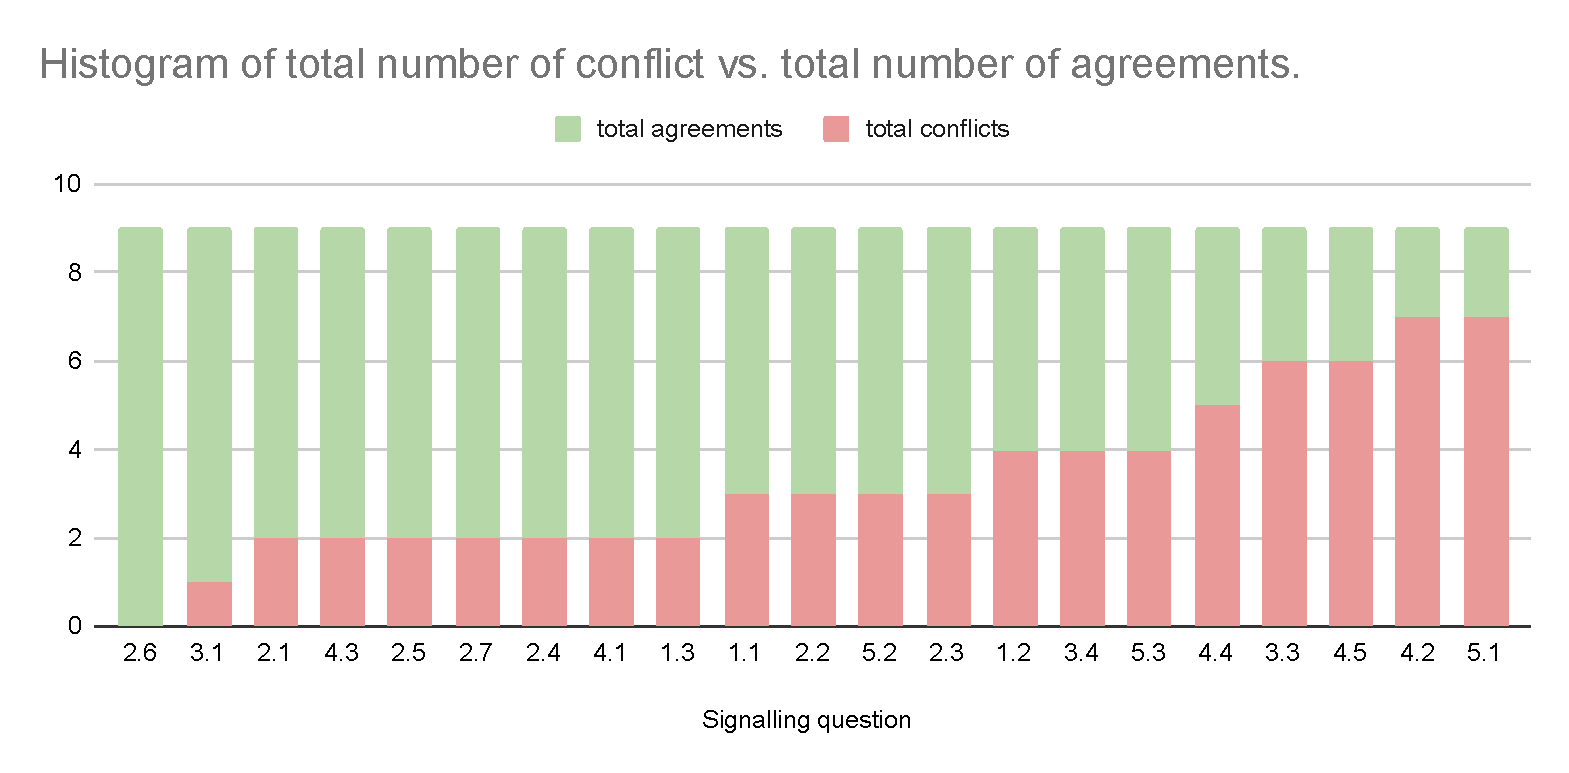
\includegraphics[width=0.99\columnwidth]{figures/agreements.pdf}
    \caption{The histogram of total number of conflicts and total number of agreements in the subset of RCTs used to calculate $\kappa_{pabak}$.}
    \label{fig:pabakagreement}
\end{figure}
%
%
%

%
%
%
% Improvements suggested by J.H.
\subsection{Feedback on Placards}
\label{disc:improv}
%
We will now address the concerns raised by a stalwart in bias assessment.
To address subjectivity arising from signaling questions 2.7 and 3.1, which inquire about the potential impact of failure to analyze participants in their randomized groups and the availability of data for all participants, respectively, we introduced the concept of a threshold.
Specifically, SQ 2.7 ``Was there potential for a substantial impact (on the result) of the failure to analyse participants in the group to which they were randomized?''.
To annotate for this question, the visual placard instructs the annotators to find the data about the number of participants included and excluded from the intention-to-treat (ITT) analysis.
The placard then goes to instructs that if more than 5\% of participants were excluded from the ITT analysis, it was a substantial number and mark this information and label it a higher risk of bias.
Similarly, for the SQ 3.1 ``Were data for this outcome available for all, or nearly all, Participants randomized?'', the term ``all, or nearly all, participants'' can be interpreted differently by different reviewers.
What one reviewer considers ``nearly all'' might be different from another reviewer's interpretation.
This ambiguity can lead to subjective judgments when applying the tool.
Therefore, we introduced the 95\% threshold meaning if the data were not available for at least 95\% or more participants, we instructed the assessors/annotators to judge the bias risk as high.
On our end, to simplify the annotation process, we chose these thresholds but enforcing a threshold deviates from the recommended RoB guidance as critiqued by this stalwart.
Thus, we must find an alternative approach to guide annotators in assessing risk without relying on thresholds.
One potential solution is to provide examples illustrating instances where low numbers may still introduce bias, offering guidance on specific result figures that annotators should scrutinize.



We also received guidance to designate specific SQ placards with a ``Subjective'' flag to signal the presence of subjective judgments.
Therefore, for several SQs, we incorporated the the recommendation added a ``subjective flag'' to the placards wherever subjective judgments were necessary.
Previously, we had marked a subjective judgment flag for the SQ 2.4 and after the recommendation we marked it also for the SQs 3.3, 3.4 and 4.5.


\textcolor{blue}{For the placard regarding 5.2, we would still need some input from Julian - we are not sure that we really understand this item within the context of a systematic review where the review authors decide on which outcome-measurement to extract. }
%
%
%
\subsection{LLM evaluation}
\label{disc:llm}
%
Manual LLM evaluation highlighted the tricky nature of bias annotation as well as the subjective nature of LLM evaluation.
LLM was tasked with the same work as human expert and was supposed to answer a SQs and extract text descriptions from RCTs that supported answer.
In some cases LLM (via ChatPDF) straightforward answered a SQ with a response option - ``Yes'' or ``No'' or ``No Information'', but in certain cases it gave an indirect answer.
For instance, in the Gleason study~\cite{gleason2015effects}, for SQ 1.1, LLM directly and correctly answered ``\textbf{Yes}, the allocation sequence was random. Extracted sentences: A random number generator (Excel, Microsoft) was used to devise a randomization series. The order of randomization was incorporated into a KEEPS database, so that treatment allocation occurred when a study identification number was assigned.''
In contrast, to answer SQ 5.2, LLM indirectly answered the following, ``Regarding RoB 5.2, the study authors reported that to correct for multiple comparisons, they divided the p-value by the number of outcomes. For example, there were five cognitive outcomes (four domain factors and one global cognition score) and six POMS mood scores. Splitting the significance value of 0.05 equally between the five cognitive and six mood sub-domains resulted in a p-value of 0.01 for each of the two primary domains investigated (cognition and mood). However, \textbf{the study authors did not provide information} on whether the numerical result being assessed was selected on the basis of the results from multiple eligible outcome measurements within the outcome domain.'' implying it found ``No Information'' for answering the SQ 5.2.


% -------------- LLM Risk Domain one --------------
LLM evaluation results for the first risk domain SQ 1.3, we saw a comparatively lower agreement between LLM and the experts because the answer to this SQ is typically found in the table text of RCT.
Text in tables is read by ChatPDF, but it might have problems correlating the correct rows and columns leading to a distorted understanding of the tables.
This could be the reason why ChatPDF sought to answer this question typically using RCT text rather than the table text wherever available.
To elaborate, for~\cite{stuck2015effect}, both the expert and LLM answered SQ 1.3 with ``No Good'', but expert used Table 2 as the evidence to answer the question while LLM used the text evidence not found in the table.

\begin{quote}
    LLM answer: No, there were no significant differences (p < 0.05; based on z-statistics from generalized estimating equation models) between the intervention and control groups in any of the baseline characteristics listed in Table 2~\cite{stuck2015effect}.
\end{quote}

The LLM correctly extracts information about participant randomization and allocation concealment procedures pertaining to answer SQ 1.1 and 1.2 leading to a rightly good $P_{O} (Extraction)$ agreements. 
As shown in the Table, for individual SQs in domain 1, $P_{O} (Extraction)$ was greater than $P_{O} (Response)$ but in an example, LLM came to a correct response judgment without correctly extracting complete evidence.
To elaborate, in~\cite{stuck2015effect}, LLM used this part of text ``'PRO-AGE Solothurn CONSORT diagram. The randomisation ratio (intervention to control group) was 1:1 in the first project phase (November 16, 2000, to March 27, 2001), and 1:2 in the second project phase (March 28, 2001, to January 8, 2002), resulting in a ratio overall of 1:1.6'' to answer SQ 1.1 with ``Yes Good'' (low risk of randomization bias) even though the extracted sentence does not contain information about the randomization method.


% -------------- LLM Risk Domain two --------------
The results for domain two where about 40\% of average $P_{O}$ agreement comes from ``No Information'' shows a lack of availability of information in RCTs for answering the SQs especially for the SQ 2.4 and 2.5.
However, in one instance for the domain 2, LLM evaluation led to identification of incorrect label from the expert. 
For SQ 2.6 in ~\cite{hassett2020digitally}, the expert had annotated this text (``The main analysis for each subgroup analysis was an interaction test in the regression models to determine whether the effect of treatment differed significantly across categories for that variable.'') to answer the question with Yes Good, but the extracted text evidence was incorrect.
LLM correctly extracted information about the intention-to-treat analysis which led to correcting the final annotation in RoBuster.



% -------------- LLM Risk Domain three --------------
The evaluation for third domain of bias brought to light the subjectivity of bias assessment. 
A lenient assessor will judge a risk of bias as low in comparison to a stringent assessor judging a bias risk as high for any SQ, but it is more pronounced in subjective SQs.
In~\cite{thorndike2014activity}, LLM and the expert used the same text evidence ``...104 (82\%) were randomized in January 2011. Five residents withdrew during Phase 1, and 99 continued participation in Phase 2...'' to answer SQ 3.1 but LLM produced the response option ``Yes Good'' and the expert rated it as ``No Bad''.
It was also because our placards have a stringent rule whereby if outcome data was not available for more than 95\% of the participants, the assessor/annotator was instructed to judge the risk as high risk of bias without considering other factors like total number of participants randomized and the kind of study.
For answering SQ 3.2 across the evaluation RCTs~\cite{myer2018integration,taylor2016novel}, the LLM was more lenient than the experts and consistently extracted information about the sensitivity analysis carried out by the study authors to account for missing outcome data, but the authors do not explicit that there was no bias due to missing outcomes data.
LLM judged signalling question 3.3 9/10 times as No information.
It questions whether the missingness in outcomes depended on its true value and is quite subjective because assessor need to contemplate on the reasons for missingness for a particular outcomes and if its true value could have affected the missingness.
For example, they need to assess whether the fact that data on falls is missing can be attributed to the actual occurrence of falls in the study.



% -------------- LLM Risk Domain four --------------
%Limitation with not mentioning what the target outcome was which confused LLM

% -------------- LLM Risk Domain five --------------
%OXO

% -------------- Comments in general --------------
%TODO: Is LLM answering the questions with ``good'' response judgment most of the time?
%We specifically observe that the expert has a more skeptical stance compared to the LLM giving lower risk judgments in several cases.
While the LLM demonstrates promise in automating RoB span extraction, additional research is necessary, particularly in the domains of prompt engineering to tackle the subjectivity inherent in SQs and the scarcity of information in RCTs required to answer SQs.
One potential avenue for improvement involves exploring the adaptation of prompting styles, such as chain-of-thought (CoT) and tree-of-thought (ToT), typically employed in language generation, for RoB text extraction task here~\cite{wei2022chain}.
%
%
%
\subsection{Limitations}
\label{subsec:limits}
%
Our study has the following limitations.
The first limitation arises from the relative scale of our annotations, with only 41 documents undergoing the annotation process.
This limitation is primarily due to financial constraints, as the availability of funds limited our ability to hire a larger number of expert annotators.
Despite the limitation, the robustness of the annotations provided by the experts remains noteworthy, as they thoroughly assessed the selected RCTs within the resources at hand.
A second limitation stems from the narrow focus of annotations, concentrated exclusively on physiotherapy and rehabilitation clinical trials.
This specificity arises from our reliance on domain experts for annotations, who possess the requisite expertise in these areas.
Though this approach inadvertently restricts the broader applicability of the annotated corpus, it guarantees high-quality annotations within the specified domains.


The LLM evaluation was limited by the fact that we chose to work with PDFs. 
There are limited platforms that interact with PDFs and this restricts our choice of the models to evaluate.
Another limitation is the stochastic nature of LLMs.
Specifically, Google Bard is freely available tool that interacts with PDFs, but we observed that the Bard results were less deterministic than ChatPDF.
Another drawback was associated with the prompts used.
The prompts employed were relatively simple and lacked information about the target outcome assessed for bias.
Consequently, for SQs seeking information on outcomes reporting for the target outcome, LLM provided general information about outcomes reported in the RCT but did not specifically consider the target outcome of interest, as it was not instructed to do so.
%
%
%
\section{Conclusion}
\label{sec:conclusion}
%
We have presented RoBuster, a new, publicly-available corpus, comprising 41 full-text RCTs richly annotated with RoB span information for 22 risk of bias questions.
The dataset fills a need for a corpus to evaluate risk of bias text span extraction using machine learning approaches.
Our corpus provides a comprehensive resource with detailed, fine-grained information, presenting individual risk of bias spans and annotator decisions on bias risk (high or low). 
We used RoBuster as a benchmark to evaluate LLMs for how well LLMs agree with human-led bias assessment.
Developed collaboratively by bias assessors and natural language processing experts, RoBuster not only supports automated approaches to bias assessment but can also contribute to Systematic Literature Review (SLR) systems.


Our work in RoB corpus annotation reaffirm the complexity of RoB assessment and the necessity of developing comprehensive instruction guidelines to increase inter annotator reliability across both tasks (assessment and annotation).
We've encountered several challenges during the development of both RoB annotation guidelines and the actual annotation attributed to how well each RCT reports the study methodology, statistical methods and outcome information along with how subjective the assessment of each RoB question is in RoB 2 tool.
In the future, we plan to refine our visual placards and extend RoBuster by adding more annotated RCT full-texts.
We also plan to test the visual annotation placards to guide trainee risk of bias assessors.
%
%
%
\section{Abbreviations}%% if any
%
\begin{enumerate}
    \item RCT - Randomized Controlled Trial
    \item RoB - Risk of Bias
    \item SR - Systematic review
    \item SQ - Signalling Question
    \item SLR - Living Systematic Review
    \item LLM - Large Language Model
    \item GPT - Generative Pretrained Transformer
    \item NLP - Natural Language Processing
    \item IAA - Inter-annotator Agreement
    \item PEDro - Physiotherapy Evidence Database RoB scale
    \item AMSTAR - A MeaSurement Tool to Assess systematic Reviews - Risk of Bias
    \item EPOC RoB - Effective Practice and Organisation of Care - Risk of Bias tool
    \item CDSR - Cochrane Database of Systematic Reviews
    \item PDF - Portable Document Format
    \item JSON - JavaScript Object Notation
    \item CoT - Chain-of-thought
    \item ToT - Tree-of-thought
\end{enumerate}
%
%
%
\backmatter

\bmhead{Supplementary information}
%
The visual placards along with detailed annotation instructions, the RCTs used in this study along with their license information, and an extended discussion section are included in the supplementary information files.
%
%
%
%\bmhead{Acknowledgments}

%Acknowledgements are not compulsory. Where included, they should be brief. Grant or contribution numbers may be acknowledged.

%Please refer to Journal-level guidance for any specific requirements.
%We thank Dr. Julian Higgins for detailed comments and improvements on our visual annotation placards that helped us further refine them post conflict resolution. 
%
%
%
\section*{Declarations}
%
\subsection*{Funding}
%
This research was supported by HES-SO, Valais-Wallis, Switzerland. 
%
%
%
\subsection*{Conflict of interest}
%
The authors declare that they have no competing interests.
%
%
%
\subsection*{Competing interest}
%
The authors declare that they have no competing interests.
%
%
%
%\subsection*{Ethics approval}
%
%Not applicable
%
%
%
\subsection*{Consent to participate and publish}
%
The experts who undertook the visual placards development and the annotation process for this corpus were explained the purpose of the annotation project and agreed to voluntarily participate in the study.
Even though they agreed to participate in the study, they can withdraw their participation any time without consequences of any kind.
They were explained the purpose and nature of the study in form of a presentation and had an opportunity to ask questions.
They were also fully informed about the purpose of the study and the eventual publication of the findings.
Each expert provided consent for the publication of the annotated corpus, along with the understanding that any identifying information would be appropriately anonymized to protect their privacy. 
%
%
%
\subsection*{Data availability}
%
Availability of data and materials on the journals preferred portal.
%
%
%
\subsection*{Code availability}
%
The notebooks used analyze RoBuster will be made public on GitHub.
%
%
%
%\subsection*{Authors' contributions}
%
%Authors' contributions
%BMC journals: \url{https://www.biomedcentral.com/getpublished/editorial-policies}
%
%
%
%%===================================================%%
%% For presentation purpose, we have included        %%
%% \bigskip command. please ignore this.             %%
%%===================================================%%
%
%\begin{appendices}
%
%
%
%\section{Annotation guidelines}\label{annot_guidelines}
%
%An appendix contains supplementary information that is not an essential part of the text itself but which may be helpful in providing a more comprehensive understanding of the research problem or it is information that is too cumbersome to be included in the body of the paper.
%
%
%
%\end{appendices}

%%===========================================================================================%%
%% If you are submitting to one of the Nature Portfolio journals, using the eJP submission   %%
%% system, please include the references within the manuscript file itself. You may do this  %%
%% by copying the reference list from your .bbl file, paste it into the main manuscript .tex %%
%% file, and delete the associated \verb+\bibliography+ commands.                            %%
%%===========================================================================================%%

\bibliography{bibliography.bib}% common bib file
%% if required, the content of .bbl file can be included here once bbl is generated
%%\input sn-article.bbl


\end{document}
